\documentclass{article}
\usepackage{graphicx} 
\usepackage{amsmath}
\usepackage{amssymb}
\usepackage{authblk}
\usepackage[skip=10pt plus3pt]{parskip}
\usepackage{csquotes}
\usepackage{url}
\usepackage{mleftright}
\usepackage{float}
\usepackage{enumitem}
\usepackage[authoryear]{natbib}
\usepackage[a4paper, margin=1in]{geometry}
\usepackage{tcolorbox}
\usepackage{enumitem}
\usepackage{caption}
\usepackage{endnotes}
\usepackage{chngcntr}
\usepackage[colorlinks=true, linkcolor=black, urlcolor=black, citecolor=black]{hyperref}


% packages required for tables generated with kable()
\usepackage{booktabs}
\usepackage{longtable}
\usepackage{array}
\usepackage{multirow}
\usepackage{wrapfig}
\usepackage{float}
\usepackage{colortbl}
\usepackage{pdflscape}
\usepackage{tabu}
\usepackage{threeparttable}
\usepackage{threeparttablex}
\usepackage[normalem]{ulem}
\usepackage{makecell}
\usepackage{xcolor}
\usepackage{setspace}

\usepackage{pifont}  % For checkmark and cross symbols
\usepackage{lmodern} % For a smoother font

% Define checkmark and cross commands with crayon-like style
\newcommand{\cmark}{\ding{51}} % Checkmark symbol from pifont
\newcommand{\xmark}{\ding{55}} % Cross symbol from 
\usepackage{verbatim}

% Increase the font size of the endnotes
\renewcommand{\enoteformat}{\normalsize\noindent\theenmark. \setlength{\parindent}{0pt}}


\setcounter{equation}{0}
\renewcommand{\theequation}{\arabic{equation}}
\DeclareMathOperator*{\var}{Var}
\DeclareMathOperator{\E}{\mathbb{E}}
\DeclareMathOperator*{\cov}{Cov}
\DeclareMathOperator*{\se}{se}
\DeclareMathOperator*{\corr}{Corr}
\newcommand{\reals}{\mathbb{R}}
\DeclareMathOperator*{\argmax}{arg\,max}
\DeclareMathOperator*{\argmin}{arg\,min}
\newcommand{\PPI}{\mathrm{PP}}

\newcommand{\mytitle}{The Mixed Subjects Design: \\ Treating Large Language Models as (Potentially) Informative Observations}

\newcommand{\mydate}{ 
}

\newcommand{\myabstract}[1]{%
\textbf{Abstract:} Large Language Models (LLMs) promise to transform the social sciences through cost-effective predictions of human behavior. However, despite growing evidence that LLMs can misrepresent such behavior, current approaches to studying causal effects with LLMs require researchers to assume that predicted and observed behavior are \textit{interchangeable}. Instead, we argue that human subjects should serve as a gold standard to correct misrepresentations within a \textit{mixed subjects design}. This paradigm offers valid and more precise estimates of causal effects at a lower cost than experiments relying solely on human subjects. We demonstrate---and extend---prediction-powered inference, a statistical method that instantiates the mixed subjects design. Our innovation is a power analysis for optimally choosing between \textit{informative but costly} human subjects and \textit{less informative but cheap} predictions of human behavior.
Mixed subjects designs could enhance scientific productivity and reduce inequality in access to costly evidence on research questions by offering valid, precise, and cost-effective inferences on causal effects and other parameters.
%Empirically, we show that the mixed subjects design reproduces the statistical precision and reproduces treatment effects of a complex experiment---even though the predicted behavior on its own does not. 
\\ \\
\textbf{Keywords:} Mixed Subjects Design, Prediction-Powered Inference, PPI Correlation, Experiments, Power Analysis, Machine Learning, Large Language Models, Moral Machine experiment, Computational Social Science
}


\title{\mytitle}
\date{\mydate}
\author{}



\begin{document}
\pagenumbering{gobble}
\maketitle


\doublespacing

\myabstract

\clearpage
\pagenumbering{arabic}
\setcounter{1}


\section{Introduction}

Large language models (LLMs)---neural networks with billions of parameters trained on massive amounts of text data---have been shown to mimic how humans respond to surveys and experimental treatments in various settings. Accurately predicting\endnote{We recognize that those deploying the methodology of ``silicon sampling'' prefer to describe LLMs used in this way as ``mimicing'' or ``modeling'' human behavior \citep{argyle_out_2023, horton2023large} instead of ``predicting'' it. We also acknowledge that there are nuanced differences between these uses for data (see, e.g., \citealt{breiman2001statistical}). However, exploring these complexities is beyond the scope of this article, and so we will stick with ``predict'' as our preferred term.} rather than observing human behavior could serve as a cost-effective and near-instantly available alternative to observing human behavior with the potential to transform the social sciences. This approach to learning about social phenomena, known as ``silicon sampling" \citep{argyle_out_2023}, might accelerate scientific progress, reduce inequities in access to costly evidence on hypotheses and research questions, and protect human subjects from deception and other risks associated with experimentation. 

However, there is scant guidance on how to leverage LLMs for conducting scientifically valid research. Researchers who currently use LLMs to predict human behavior have to rely implicitly or explicitly on what we term the \textit{interchangeability assumption}, a general premise that researchers adopt when drawing conclusions from predictive models of social processes rather than observations thereof (e.g. \citealp{friedman_methodology_1953}). When predicting human behavior, this assumption implies that the data extracted from LLMs closely correspond to human behavior or the responses given in a survey. The underlying logic of this approach is to treat silicon subjects \textit{as if} they were human participants. This assumption leads to valid inference only if the predicted responses approximate---at least on average---the same parameter estimate as from the human subjects.

Unfortunately, there is growing evidence that LLMs inaccurately portray human behavior (\citealp{Bisbee2024synthetic, park2024diminished, takemoto_moral_2024, abdurahman2024perils}). Even in settings where LLMs happen to accurately predict human behavior, there is a lack of generalizable procedures, metrics, and conventions to assess when this approximation is sufficiently accurate to be used in traditional null hypothesis testing. Currently, the interchangeability of predicted and observed behavior is assessed empirically on a case-by-case basis. As a result, silicon sampling is of minimal practical benefit since human subjects data must be collected alongside LLM predictions at a scale sufficient to validate the interchangeability assumption. Some have therefore suggested that predictions be confined to exploratory stages of research, such as LLM-powered pilot studies for anticipating effect sizes \citep{grossmann_ai_2023,ashokkumar_predicting_2024}.

To address this gap, we propose a \textit{mixed subjects} approach to designing research with LLMs. Rather than outright rejecting the assumption that human behavior and LLM predictions are interchangeable a priori, we argue that data from human subjects should inform inferences drawn from LLMs in a coherent statistical framework. We propose that observations from human subjects can be leveraged as a gold standard to correct for misrepresentations of human behavior through LLMs. We demonstrate how to implement this approach with prediction-powered inference (PPI) \citep{angelopoulos_prediction-powered_2023-1, angelopoulos2024ppi}, a recent statistical method that instantiates the mixed subjects approach. PPI allows researchers to combine observations of human behavior with predictions of that behavior generated by LLMs or other algorithms. So long as there is a correspondence between predicted and observed behavior, PPI produces valid point estimates with narrower confidence intervals than those derived solely from human subjects.

LLMs introduce a trade-off between predicted and observed behavior when estimating parameters such as causal effects. While obtaining predictions from LLMs is more cost-effective than recruiting human subjects, these predictions are less informative for estimating parameters than directly observed behavior. We derive a power analysis that formalizes and resolves this trade-off by balancing the costs of collecting these two types of data with the extent they inform inferences on parameters. Our power analysis allows researchers to allocate a fixed research budget to an optimal mix of human subjects and predictions that maximizes statistical power. Alternatively, researchers can minimize costs with an optimal combination of human subjects and predictions to achieve a given level of power. These functionalities will be integrated into the PPI Python library, available at \href{https://github.com/aangelopoulos/ppi_py}{https://github.com/aangelopoulos/ppi\_py}. With the extension of a power analysis, PPI becomes a fully usable methodology for conducting mixed subjects studies. 

This article demonstrates how researchers can use LLMs not only in exploratory but also in confirmatory research. The mixed subjects design with PPI ensures the validity of point estimates while allowing researchers to achieve higher precision at a lower cost than with human subjects alone. Therefore, the mixed subjects design may provide many of the benefits of silicon sampling while avoiding its drawbacks. 


\section{The Silicon Subjects Design}

Experiments in surveys, labs, and the field significantly enhanced our understanding of causal processes in the social sciences. However, experiments also face limitations, including the costs of conducting research, recruitment of harder-to-reach participants, and issues of measurement and generalizability. Below we outline how the silicon subjects approach promises to address these issues and highlight the potential pitfalls. 

\subsection{Promises of the Silicon Subjects Design}\label{sec:promises-silicon}

The silicon subjects design asserts that LLMs can mimic the behavior of human participants in empirical studies based on a prompt given by the researcher. In the context of experiments, the prompt contains the experimental manipulation, with silicon subjects being randomly assigned to a condition. The prompt may also include a profile of study participants with demographics, attitudes, and other information. While such a profile is necessarily an incomplete representation of a participant, it allows researchers to create a ``silicon sample" \citep{argyle_out_2023} that matches the demographic makeup of the population of interest. The additional context provided to the LLM may increase the diversity of responses one would expect in a human population or even increase the LLM's accuracy in predicting behavior \citep{gui2023challenge}. 
Based on successful replications of canonical experiments with the silicon subjects design, some scholars concluded that LLM predictions were interchangeable with human behavior under certain conditions:
\begin{displayquote}
\textit{These findings could indicate that—at least in some instances—GPT-3 is not just a stochastic parrot and could pass as a valid subject for some of the experiments we have administered.} (\citealp{binz2024using}: 9)
\end{displayquote}
\begin{displayquote}
\textit{Practically speaking, LLMs may be most useful as participants when studying specific topics, when using specific tasks, at specific research stages, and when simulating specific samples.} (\citealp{dillion2023can}: 597)
\end{displayquote}
If silicon subjects could substitute human participants, LLMs may help overcome the limitations of experiments that exclusively draw on responses from human subjects. The first set of issues relates to the cost of conducting experiments with human subjects. Depending on wages paid to survey participants and fees for using online survey panels, a single survey response can cost several dollars. Typical survey experiments in the social sciences require significant numbers of survey participants to identify an effect. For example, researchers need a sample size of $n=6,570$ to have a 90\% chance of detecting an effect of size $d=0.08$ with a two-sided $t$-test at $\alpha=0.05$ (Figure \ref{fig:gpower-power-analysis} in the Supporting Information). While $d=0.08$ represents the median effect size in a high-quality sample of online survey experiments in the social sciences \citep{rauf_audit_2024}, the required number of participants is even higher for smaller effects. Larger sample sizes are also required for experiments that systematically assess a broad range of hypotheses \citep{dellavigna_what_2018,milkman_megastudies_2021,voelkel_megastudy_2023, tappin_quantifying_2023} and those aimed at estimating interaction effects \citep{gelman_you_2018}. Across these cases, the costs of recruiting a sufficient number of human subjects may be prohibitive for researchers with more limited budgets. Silicon sampling offers a cost-effective alternative to human respondents. The cost of predicting a survey response with an LLM with currently available APIs can be as low as a fraction of a cent (Table \ref{tab:model-overview}). 

A second set of issues relates to challenges in finding suitable participants for a study. While researchers often go to significant lengths to create a sample representative of a target population, certain participants remain hard to reach on a typical panel for online research \citep{chandler_online_2019}. For instance, typical online panels for survey research consist of younger, more liberal, and more educated respondents who more are more likely to be White and who earn less on average than the American population \citep{berinsky_evaluating_2012, levay_demographic_2016, zack_can_2019}. Collecting samples that are representative across multiple dimensions---such as age, gender, income, and education---can be challenging since combinations of these characteristics may be rare among participants available on an online panel. If accurate, silicon sampling allows researchers to collect more observations on these otherwise hard-to-reach populations, with observations being nearly instantly available. Silicon subjects may even serve as alternative study populations if ethical concerns and risks limit the number of participants that can be recruited for experiments \citep{grossmann_ai_2023,bail_can_2024}.   

Finally, experimental research, like other quantitative scholarship, is only as good as the quality of measurements taken. Limited attention spans, insufficient effort, participant attrition, and non-compliance with research protocols are just a few examples of undesirable behaviors by study participants \citep{stantcheva_how_2023}. While these features characterize the \textit{typical} participant, silicon sampling envisions the \textit{ideal} participant---a prediction algorithm that exhibits human-like behavior but which allows researchers to control how much the responses randomly vary from one prompt to another, explicitly defining how erratic silicon subjects should behave. It may be unrealistic but advantageous to prompt LLMs to be inhumanely consistent in their responses and strictly abide by the researchers' directions \citep{grossmann_ai_2023}. Proponents of the silicon sampling approach could even argue that unrealistic distributions of LLM predictions help estimate parameters. While predictions of human responses exhibit less variability than human responses \citep{Bisbee2024synthetic,mei2024turing}, it may be precisely this misrepresentation that allows for more precise measurement of central tendencies such as the mean. This property does not imply that researchers obtain an accurate parameter estimate, but that this estimate exhibits less statistical uncertainty than an estimate obtained from a sample of human subjects.

\subsection{Perils of the Silicon Subjects Design}\label{sec:perils-silicon}

Empirical studies question whether silicon subjects alone will be sufficient to draw valid conclusions about human behavior. Predictions of human behavior have been shown to systematically diverge from observed behavior. For example, \cite{atari_xue_park_blasi_henrich_2023} find that LLMs respond to various tasks more like those from western, educated, industrialized democracies than those from other parts of the world. \cite{alvero2024large} find that LLMs, when compared to actual college applicants, write college admissions essays most similarly to those who are male and from neighborhoods with high socioeconomic status. When researchers are interested in populations or tasks that LLMs are less able to mimic, silicon sampling may lead them astray. 

Sources of prediction error are manifold and it remains unclear which ones can resolved. LLMs may inaccurately predict outcomes of certain groups of individuals because these have been misrepresented or underrepresented in the models' training data \citep{wang_large_2024,bail_can_2024}. While improving the representativeness and overall quality of the training data may enhance prediction accuracy, improving the inputs to LLMs may not be sufficient to rule out errors stemming from the prediction algorithm itself. LLMs have been shown to respond differently depending on the order of a question or give the same answer consistently \citep{park2024diminished}. Errors may also arise from the complexity of the research design. While LLMs achieved remarkable accuracy in predicted responses to social surveys \citep{kim_ai-augmented_2024}, predicting responses to experimental stimuli and more complex prediction tasks may result in higher error rates. At a more fundamental level, it remains unclear whether LLM predictions can be trusted without validation against human respondents. A treatment effect estimated based on LLM predictions could be a statistical fluke or an effect that would replicate in studies with human subjects  \citep{harding2023ai}.

Parameter estimates based on LLM predictions may not only be incorrect but also misleadingly precise. For example, using LLMs to generate many predicted values for an outcome $Y$ and regressing these on an independent variable $X$ results in narrow confidence intervals for a parameter simply because standard errors shrink with sample size. However, if LLMs inaccurately predict human behavior, the point estimates misrepresent the relationship between $Y$ and $X$ that would be observed in a sample of human subjects. Therefore, silicon samples may create a false sense of precision, leading to overly narrow confidence intervals with incorrect centers. This issue parallels the analysis of Big Data from non-representative samples, where researchers risk being ``precisely inaccurate" (\citealp{mcfarland_big_2015}). If biases are not adequately addressed, the availability of large and inexpensive data sources may do more harm than good \citep{meng_statistical_2018,bradley2021unrepresentative}. For example, silicon samples could further amplify doubts about the replicability of findings from experimental social science (c.f. \citealp{freese_emergence_2018}), not because studies lack sufficient statistical power to discern true effects from false positives, but because they are sufficiently powered to detect \textit{any} effect.


\section{The Mixed Subjects Design}

We propose the mixed subjects design, an alternative to silicon sampling and an umbrella term for statistical methods that provide valid inferences about human behavior while maintaining the benefits of employing silicon subjects. The mixed subjects approach treats silicon subjects as \textit{potentially} informative of human behavior, relying on the interchangeability assumption to an intermediate degree and in a way that is subject to disconfirmation via empirical evidence. Human respondents count as a gold standard to correct potentially flawed predictions from LLMs. The goal is to build confidence in LLMs as a research tool by combining human and silicon subjects with statistical methods that produce valid parameter estimates while maintaining the benefits of low costs of LLM predictions and increased statistical power to detect treatment effects. 
In the following, we present prediction-powered inference \citep{angelopoulos_prediction-powered_2023-1}, a recent statistical framework that instantiates the mixed subjects approach.
\clearpage

\begin{figure}[p]
    \centering
    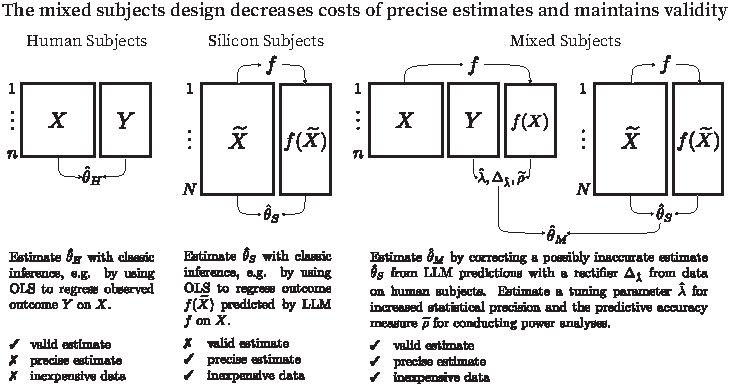
\includegraphics[width=1\linewidth]{0_Infogram_v4.pdf}
    \caption{Comparison of experiments with human, silicon, and mixed subjects designs}
    \label{fig:concept}
\end{figure}

\clearpage

\subsection{The Mixed Subjects Design with PPI}\label{sec:PPI}

Prediction-powered inference (PPI) is a statistical method that combines a dataset of ``gold-standard" observations with predictions from a machine learning algorithm to estimate a broad class of estimands, including population means, regression coefficients, and quantiles  \citep{angelopoulos_prediction-powered_2023-1,angelopoulos2024ppi}. PPI does not make assumptions about the accuracy of the machine learning algorithm used to predict the dependent variable. Instead, the predictions are treated as informative but imperfect proxies. PPI uses the gold-standard observations to estimate prediction error and adjust parameter estimates accordingly. These corrected estimates target the same population parameters as a classical experiment (e.g. a regression coefficient estimated with a sample of responses from human subjects). Yet the PPI estimates are also more precise since increasing sample size with machine learning predictions leads to narrower confidence intervals. In the PPI framework, predictions and gold-standard observations thus complement each other in obtaining valid and precise point estimates.

To explain PPI in more detail we will follow the notation in \citet{angelopoulos_prediction-powered_2023-1,angelopoulos2024ppi}. To estimate a parameter $\theta$, PPI requires three things---a gold-standard (or labeled) dataset $\{(X_i, Y_i)\}_{i=1}^n$, an unlabeled dataset $\{\widetilde{X}_i\}_{i=1}^N$, and a machine learning algorithm $f$ that maps $X$ to a prediction of $Y$. PPI applies the machine learning algorithm to both datasets---this gives $\{(X_i,Y_i,f(X_i))\}_{i=1}^n$ and $\{(\widetilde{X}_i, f(\widetilde{X}_i))\}_{i=1}^N$.  
To understand how PPI estimates a parameter $\theta$ with these two datasets, it is instructive to consider how PPI estimates the simple population mean, e.g. the average student test score, loan amount, or time spent on social media (Equation \ref{eq:ppi-mean}, see also Figure \ref{fig:concept}). 


\begin{equation}\label{eq:ppi-mean}
    \hat{\theta}^\PPI = \underbrace{\frac{1}{N} \sum_{i=1}^N \hat \lambda f(\widetilde{X}_i)}_{\displaystyle \huge \hat \lambda \hat \theta_S} - \underbrace{\left( \frac{1}{n} \sum_{i=1}^n\hat \lambda f(X_i)- \frac{1}{n} \sum_{i=1}^n Y_i\right)}_{\displaystyle \huge \hat \Delta_{\hat \lambda} = \hat \lambda \hat  \theta_{f(X_i)}- \hat \theta_H} 
\end{equation}

The estimand $\hat{\theta}^\PPI$ comprises two parts: the estimand based on the algorithm's predictions $\hat \theta_S$ and a rectifier $\hat \Delta_{\hat \lambda}$. The rectifier quantifies the difference between the predicted and observed values from the gold-standard dataset and uses this information to adjust the estimate obtained from the prediction algorithm. If the algorithm is very accurate, the rectifier will be close to zero and the estimate is largely based on predictions. To optimize statistical precision, PPI estimates $\lambda$, an additional tuning parameter ranging from $0$ to $1$. $\hat \lambda \approx 1$ implies that full weight is given to the predictions whereas $\hat \lambda \approx 0$ means that the estimate is mostly based on the gold-standard observations.

In a mixed subjects experiment, the human subjects represent the gold standard dataset $\{(X_i, Y_i)\}_{i=1}^n$. The variable $X_i$ encodes the demographic covariates and the treatment assignment of the $i$th human subject. The variable $Y_i$ is the response from the $i$th human subject. For the unlabeled dataset $\{\widetilde{X}_i\}_{i=1}^N$ we create $N$ silicon subjects, for example by obtaining a representative sample of the target population \citep{argyle_out_2023}. For a silicon sample with covariates $\widetilde{X}$, we turn the information in $\widetilde{X}$ into a prompt for an LLM, resulting in a predicted survey response $f(\widetilde{X})$. Prompting the LLM for both the human and silicon subjects gives the datasets $\{(X_i, Y_i, f(X_i))\}_{i=1}^n$ and $\{(\widetilde{X}_i, f(\widetilde{X}_i))\}_{i=1}^N$. Researchers can then compute point estimates and confidence intervals with these two datasets using the software provided by \citet{angelopoulos_prediction-powered_2023-1, angelopoulos2024ppi}.

To apply PPI to a mixed subjects experiment, we need to verify several assumptions. First, PPI requires the classical assumption that $\{(X_i,Y_i)\}_{i=1}^n$ are independent and identically distributed (i.i.d). In addition, PPI requires that $\{\widetilde{X}_i\}_{i=1}^N$ are i.i.d. and that $\{ \widetilde{X}_i\}_{i=1}^N$ are drawn from the same distribution as $\{X_i\}_{i=1}^n$. That is, the hypothetical demographics of the silicon subject population must match the demographics of the human subject population.  Likewise, the treatment assignment mechanism must be the same for both groups. Ideally, each silicon subject should correspond to a human subject who would have been surveyed had the sample size $n$ been larger.
Second, PPI requires that the training of the machine learning algorithm $f$ is independent of both datasets. This assumption may be violated when the data from human subjects has been previously published and included in the LLM's training data. Finally, the procedure of prompting the LLM must be the same for the gold standard and the unlabeled dataset. This means that the same parameters and model should be used on both datasets. Likewise, the method used to turn the demographic and treatment information into a prompt must be the same for both datasets.

\subsection{The PPI Correlation}

In section \ref{sec:perils-silicon}, we argued that using classical inference methods---such as regression---to estimate parameters with a large number of predictions of human behavior gives a false sense of precision. Even if LLMs inaccurately portray human behavior, point estimates derived from their predictions exhibit too little uncertainty.
Therefore, a study design that treats LLM predictions not as interchangeable with human subjects must account for how closely LLMs can predict behavior. Therefore, we derived the \emph{PPI correlation} $\tilde{\rho} \in [-1,1]$ as an empirical measure of the interchangeability assumption. The PPI correlation $\widetilde{\rho}$ measures the correlation between the classical estimator $\hat{\theta}_{H}$ based on human subjects and the estimator $\hat{\theta}_S$ based on the LLM predictions.\endnote{Hence, the PPI correlation $\tilde{\rho}$ does not directly refer to the correlation between predicted and observed values of the dependent variable. The PPI correlation $\widetilde{\rho}$ is defined mathematically in equation~\eqref{eq:PPI_corr} in the Supporting Information.} To demonstrate that $\tilde{\rho}$ measures interchangeability, we derived an \textit{effective sample size}. The effective sample size in a mixed subjects experiment is the sample size required to achieve the same standard error for a parameter as in a human subjects experiment, allowing for a direct comparison of the two types of data. In section \ref{sec:effective-sample-size} of the Supporting Information, we show that the effective sample size when using PPI is given by
\begin{equation}\label{eq:n0}
    n_0 = n\cdot\frac{n+N}{n+N-N\tilde{\rho}^2},
\end{equation}
where $n$ and $N$ are the number of human and silicon subjects in the mixed subjects experiment and $n_0$ is the sample size in an equivalent human subjects experiment. 
When $\tilde{\rho}=1$, the effective sample size is $n+N$ and human and silicon subjects are treated as equally informative. When $\tilde{\rho}=0$, the effective sample size is $n$ and only human subjects are used. In empirical applications, $\tilde{\rho}$ will likely be between $0$ and $1$, indicating that the prediction algorithm is informative but not as informative as human subjects for estimating a parameter.
For example, if the PPI correlation is $\tilde{\rho}=0.75$ and $N/n=5$ so that for every human subject there are 5 silicon subjects, conducting a mixed subjects experiment PPI is equivalent to a human subjects experiment with 88\% more participants. As such, $\tilde{\rho}$ quantifies how informative predictions are in estimating $\theta$ and measures the extent to which predictions are interchangeable with gold standard data. 

In the following, we show that higher values of the PPI correlation are crucial for obtaining smaller standard errors for parameters, implying narrower confidence intervals, higher statistical power, and lower costs of conducting mixed subjects experiments relative to human subjects experiments. 
%$\tilde{\rho}$ does not directly refer to the correlation between observed and predictions but the quality of the predictions in estimating $\theta$. 
As shown in section \ref{sec:ppi-se-and-corr} of the Supporting Information, the PPI standard error can be written as 

\begin{equation}\label{eq:PPI-se}
    \mathrm{SE}(\hat{\theta}^{\PPI}) = \frac{\sigma}{\sqrt{n}}\sqrt{1 - \frac{N}{N+n}\tilde{\rho}^2},
\end{equation}

where $\sigma/\sqrt{n}$ is the standard error of $\hat{\theta}_H$ in an experiment with $n$ human subjects. As $\tilde{\rho}$ is always between $-1$ and $1$, the standard error of $\hat{\theta}^{\PPI}$ is always less than the classical standard error $\sigma/\sqrt{n}$. A smaller standard error for $\hat \theta^\PPI$ implies that a mixed subjects design with PPI produces narrower confidence intervals and higher statistical power than a human subjects experiment. Figure \ref{fig:theo-ppi-classic-ci} illustrates how achieving this higher statistical precision depends on $\tilde{\rho}$ and on the ratio $N/n$. The PPI standard error becomes narrower than the classical standard error for larger $N$ relative to $n,$ and this benefit is greatest for higher values of the PPI correlation. For example, if $N/n = 5$ and $\tilde{\rho} = 0.5$, then the PPI standard error will be approximately $11\%$ smaller than the classical standard error since $\sqrt{1-(N/(N+n))\tilde{\rho}^2} \approx 0.89$. If $\tilde{\rho}$ increased to $0.75$ and the same sample sizes were used, the PPI standard error would be approximately $27\%$ smaller than the classic standard error. The same consideration applies to confidence intervals since the ratio of standard errors is equivalent to the ratio of the width of confidence intervals. Finally, higher values of $\tilde{\rho}$, implying a smaller standard error, result in a non-linear increase in statistical power.

\clearpage

\begin{figure}[p]
    \centering
    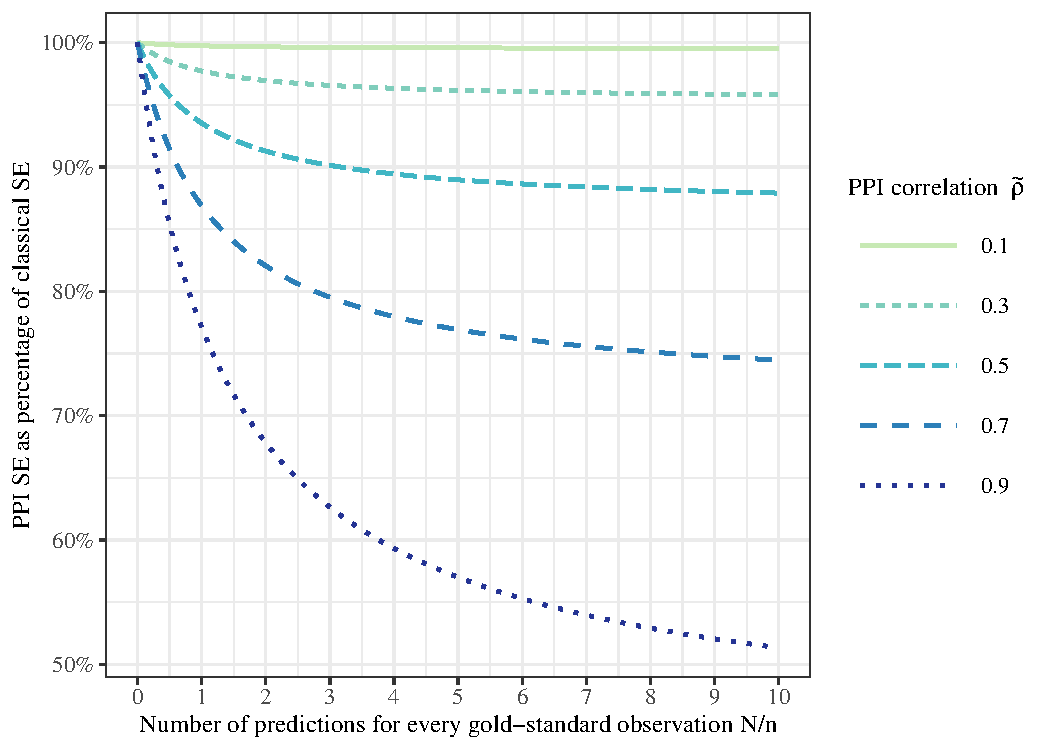
\includegraphics[width=0.8\linewidth]{3_SeAsPercentageOfShareOfClassicSe.pdf}
    \caption{The x-axis shows the ratio $N/n$ of samples sizes with $N$ predictions $f(X_i)$ and $n$ gold standard observations $Y_i$. The y-axis shows the ratio of the PPI standard error to the classical standard error, defined by $\sqrt{1-(N/(N+n))\tilde{\rho}^2}.$ 
    }
    \label{fig:theo-ppi-classic-ci}
\end{figure}
\clearpage

The PPI standard error directly depends on $\tilde{\rho}$, the ratio of silicon subjects to the total sample size $N/(N+n)$, and the standard error of the classical estimator $\sigma/\sqrt{n}$. As shown in Figure \ref{fig:theo-ppi-classic-ci}, including more silicon subjects is most effective in reducing standard errors when the PPI correlation $\tilde{\rho}$ is closer to $1$. Hence, researchers can maximize returns on predictions by using algorithms that accurately portray human behavior. Researchers could increase $\tilde{\rho}$ by choosing more accurate prediction algorithms. These may include LLMs with more parameters, those trained on higher-quality data, models fine-tuned for specific prediction tasks, or models with retrieval-augmented generation \citep{lewis_retrieval-augmented_2021}. Prompt engineering---such as providing more context, examples, or specific instructions---may also enhance prediction accuracy. 

\subsection{PPI Power Analysis}\label{sec:PPI power}

Power analyses allow researchers to determine the necessary sample size for a desired level of power---i.e., the probability of correctly rejecting the null hypothesis when there is an effect \citep{cohen_statistical_1988}.  A power analysis not only addresses the practical question of how many resources researchers need to invest to find a significant effect but is also instrumental in advancing science. True treatment effects, particularly small ones, may go unnoticed if the sample size is too small. Reporting false negatives impedes researchers in discerning sound from flawed explanations for social phenomena, thwarts the accumulation of knowledge, and may explain the existence of inconsistent findings on core concepts in the social sciences \citep{thye_reliability_2000,stadtfeld_statistical_2020}. Power analyses are therefore crucial for testing and advancing theory. Yet no such method has been developed for PPI. To address this gap, we derive a power analysis, completing the toolkit necessary for conducting mixed subjects experiments.

Our power analysis for the mixed subjects design is based on the trade-off between human and silicon subjects. Obtaining a silicon sample is much more affordable than recruiting human subjects. However, silicon subjects are generally less informative than humans when estimating a parameter, corresponding to a PPI correlation of $\tilde{\rho} < 1$ when human and silicon subjects are not interchangeable. 
Researchers can make an optimal choice for combining a sample size of human subjects $n$ with $N$ silicon subjects, and this combination depends on the PPI correlation $\tilde{\rho}$, a hypothesized effect size, a desired level of power, the cost of recruiting human and silicon subjects, and the available research budget. Given these parameters, our power analysis allows researchers to optimally decide between recruiting \textit{costly but informative} human subjects or \textit{less informative but cheap} silicon subjects.
This multidimensional choice problem can be solved with constraint optimization \citep{apostol_calculus_1969}, allowing researchers to answer the following two questions.

First, which pair of sample sizes $(n, N)$ yields the highest power given a hypothesized effect size, fixed research budget, the cost of recruiting silicon subjects relative to human subjects, and how informative LLMs are in predicting human behavior $\tilde{\rho}$? Researchers may be particularly interested in finding the \textit{most powerful pair} $(n, N)$ if a limited research budget is the main constraint and resources should be allocated most effectively to maximize power. Figure \ref{fig:powerful-cheapest-pair}a illustrates this optimization problem: Finding the most powerful pair involves selecting combinations of $n$ and $N$ that satisfy the budget constraint and identifying the point where statistical power is highest.
Second, which combination of sample sizes $(n, N)$ is the cheapest to sample for a desired level of power, an effect size, the costs of silicon relative to human subjects, and the PPI correlation $\tilde{\rho}$? Researchers might be more interested in this question if budget constraints are less salient but resource allocation should still be as efficient as possible. Identifying the \textit{cheapest pair} means selecting the combination $(n, N)$ that gives a desired level of power and identifying the point where the cost is lowest (Figure \ref{fig:powerful-cheapest-pair}b). 

\clearpage
\begin{figure}[p]
    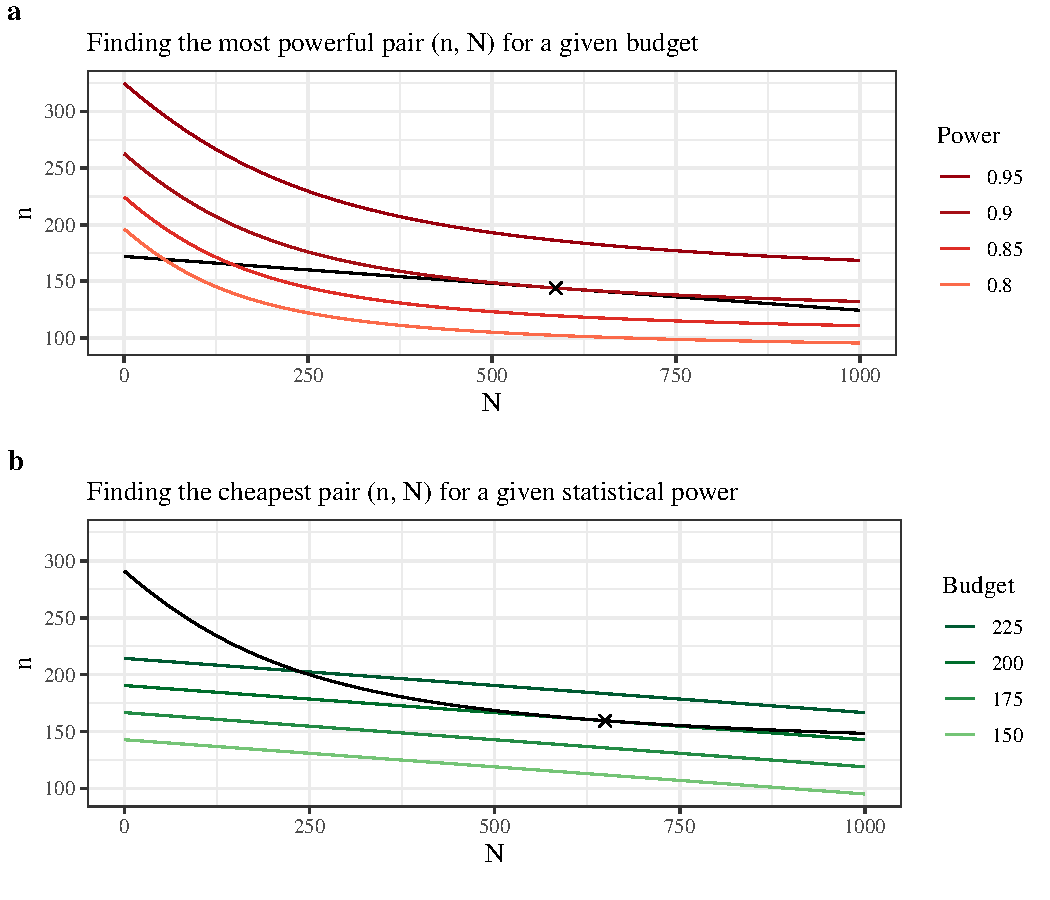
\includegraphics[width=1\linewidth]{9_MostPowerfulAndCheapestPair.pdf}
    \caption{Illustration of the constraint optimization with $\tilde{\rho}=0.75$, effect size $\delta = 0.2$, classical standard error $\hat \sigma/ \sqrt{n} = 1$, and a ratio of the costs of sampling silicon subjects to human subjects $\gamma=0.05$ (\textbf{a}) Given a fixed budget, the PPI power analysis identifies the combination of sample sizes $(n, N)$ with the highest statistical power. (\textbf{b}) Given a desired level of statistical power for detecting an effect, the PPI power analysis identifies the combination of sample sizes $(n, N)$ that minimizes budget expenditure.}
    \label{fig:powerful-cheapest-pair}
\end{figure}
\clearpage

Statistical software published alongside this article offers user-friendly tools for conducting power analyses in mixed subjects studies with PPI. 
This power analysis is \textit{data-driven} in that $\tilde{\rho}$ needs to be estimated from a small dataset $\{(X_i, Y_i, f(X_i))\}_{i=1}^n$. Researchers could also test hypothetical values for $\tilde{\rho},$ reflecting more or less accurate prediction algorithms. However, applying the PPI software is required to obtain precise estimates. Details on the derivation of the PPI power analysis are given in sections \ref{sec:most-powerful-pair} and \ref{sec:cheapest-pair} of the Supporting Information. 

\subsection{Lowering Costs of Data Collection}

PPI produces narrower confidence intervals and higher statistical power than classical inference. Whether PPI is also more cost-effective depends on the PPI correlation $\tilde{\rho}$ and $\gamma$ --- the ratio of the costs of surveying silicon and human subjects. That is,
\begin{equation}
    \gamma = \frac{c_f}{c_Y},
\end{equation}
where  $c_f$ is the cost of prompting an LLM to give a prediction, and $c_Y$ is the cost of surveying a human subject. In section \ref{sec:power} of the Supporting Information, we show that PPI is more cost-effective than classic inference with human subjects if and only if 
\begin{equation}\label{eq:cost-saving-condition}
\tilde{\rho}^2 > \frac{4 \gamma}{(1+\gamma)^2}.
\end{equation}

For example, we could assume a cost of \$3.20 for a participant to fill out a 12-minute survey, paying participants the 2024 California minimum wage of \$16.00/hour. Based on the costs of \$0.003 for prompting an LLM for this study, we calculated that any $\tilde{\rho}>0.06$ would be sufficient for PPI to save costs when compared to classical inference with human subjects only. More generally, if condition \eqref{eq:cost-saving-condition} is satisfied and researchers use the optimal sample size from the PPI power analysis, conducting mixed subjects can be substantially more cost-effective than experiments with human subjects only. Figure \ref{fig:perc-cost-reduction} shows that PPI experiments become less expensive than classical experiments as predictions become more affordable, with substantial savings at higher values of the PPI correlation. This theoretical result carries important implications as the field of generative AI continues to advance. The costs of conducting mixed subjects experiments will further decrease relative to classical experiments as costs for prompting LLMs decrease (e.g.  API fees) and LLMs become more capable of predicting human behavior. 

\clearpage

\begin{figure}[p]
    \centering
    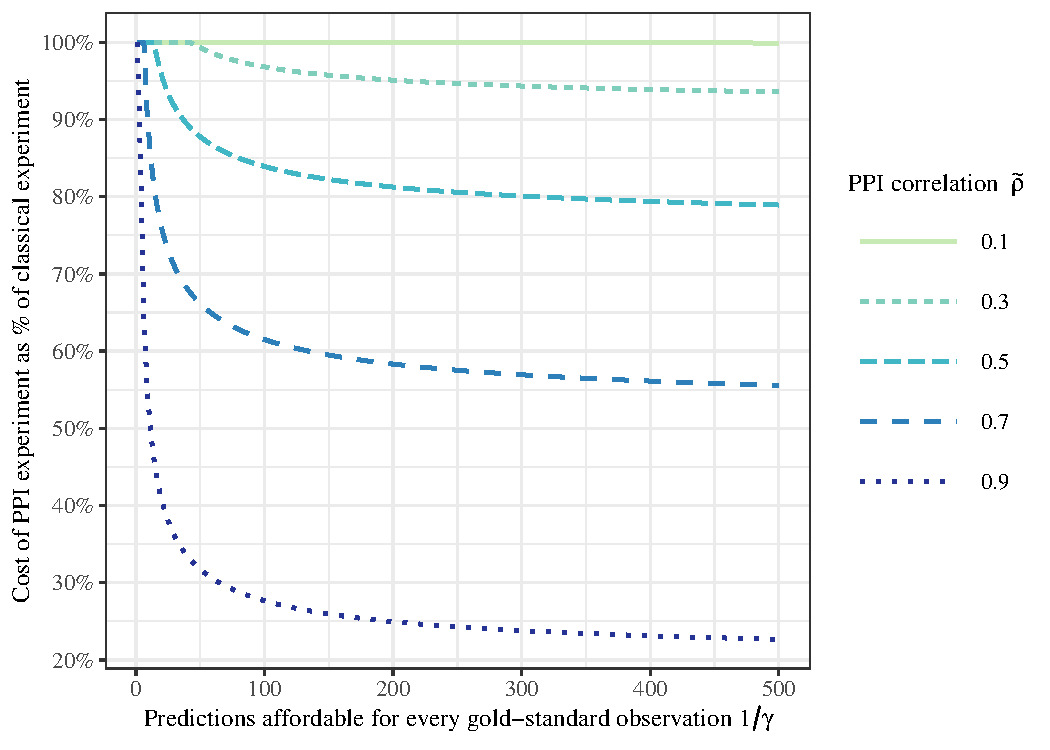
\includegraphics[width=0.8\linewidth]{3_PercentCostOfHumanSubjectsExperiment.pdf}
    \caption{The y-axis shows the costs of conducting a mixed subjects experiments with PPI as a percentage of the costs of conducting a classical experiment with human subjects only, given by $1 - \tilde{\rho}^2(1 - \gamma) + 2 \sqrt{\gamma \tilde{\rho}^2(1-\tilde{\rho}^2)}$, as a function of the PPI correlation $\tilde{\rho}$ and the number of silicon subjects that researchers can afford for the costs of recruiting a human subject $1/\gamma = c_Y/c_f.$}
    \label{fig:perc-cost-reduction}
\end{figure}

\clearpage


\section{Application to the Moral Machine Experiment}

The Moral Machine experiment \citep{awad_moral_2018} sought to better understand the factors influencing people's decisions in moral dilemmas that self-driving cars might face on the road. In this conjoint experiment, participants were presented with hypothetical scenarios where a sudden brake failure would result in harm to either passengers or pedestrians. Participants could only spare one of the two groups. If participants choose to save the passengers, the autonomous vehicle would drive through a crosswalk where pedestrians are crossing the street. If participants chose to spare the pedestrians instead, the car would crash into a concrete barrier. The experiment measured how attributes such as age, gender, social status, and the number of individuals influenced the probability of participants choosing to save one group over the other. Using a weighted simple linear regression, \citet{awad_moral_2018} estimate the Average Marginal Component Effect (AMCE). The AMCE represents the causal effect of an attribute of a moral dilemma on a respondent's decision to spare passengers or pedestrians.
 
Our main interests in this application of PPI with LLMs are (\textbf{a}) to assess the extent to which including LLM predictions increases statistical precision and (\textbf{b}) to compare the validity of point estimates from PPI to those derived from LLM predictions. Analogous to Figure \ref{fig:theo-ppi-classic-ci}, we define increases in precision as the percent reduction in the width of the PPI confidence intervals relative to the width of the confidence interval obtained from human subjects only. We define the validity of a point estimate by the percent of confidence intervals that cover the true causal effect in a specific population. While such population parameters remain of course unknown, we use a quota sample of Americans who responded to the Moral Machine experiment to obtain best possible estimates of the true AMCEs (Figure \ref{fig:amce-estimates}). These AMCEs serve as a benchmark for comparing the validity of silicon sampling and the mixed subjects design with PPI. 

\subsection{Methods}

\citet{awad_moral_2018} obtained a convenience sample with millions of decisions on moral dilemmas from participants worldwide. We used the subset of 492,921 participants who completed an optional demographic survey to obtain a sample of the American population. Using quotas on age, education, gender, and income from the 2016 American Community Survey \citep{acs_2016}, we randomly sampled 2,097 Americans who evaluated a total of $22,315$ moral dilemmas.
Our sample closely resembles the demographics of the United States, except for older individuals, who could not be sufficiently sampled due to their minimal presence in the Moral Machine experiment (Figure \ref{fig:demographic-distribution}).

Next, we created the prompts for the LLMs based on the replication data from the Moral Machine experiment. The replication data records the attributes of the moral dilemmas evaluated by survey participants, such as the number of passengers in the car. We converted this numerical representation into a text description of the dilemmas with computer code adapted from a related study \citep{takemoto_moral_2024}. We also added a demographic profile to the prompt, including the age, education level, gender, and income of the survey respondent who evaluated the dilemma. Please refer to section \ref{sec:appendix-moral-machine} in the Supporting Information for an example. We then used the OpenAI API to prompt four LLMs---GPT4 Turbo (gpt-4-turbo), GPT4o (gpt-4o), and GPT3.5 Turbo (gpt-3.5-turbo-0125)---to predict the decisions of these survey respondents for the moral dilemmas.

We then compared the validity and statistical precision of point estimates derived from PPI against a naive approach that pools human and silicon subjects by incrementally increasing the number of silicon subjects. From the quota sample of 2,097 Americans, we randomly selected $n=500$ human subjects and added $n\times k =N$ silicon subjects for $k=(.25, .5, .75, 1, 1.5, \dots,4.5,5)$. For each combination of sample sizes $n$ and $N=(125,250,...,2500)$, we repeated the sampling 300 times and calculated the mean width and coverage of the confidence intervals. We estimated the AMCE for each scenario attribute with a weighted simple linear regression \citep{hainmueller_causal_2014}. To assess the validity and precision of the naive approach, we applied the weighted simple linear regression to the pooled sample of size $n+N$. We used the Python library created by \citet{angelopoulos_prediction-powered_2023-1, angelopoulos2024ppi} to obtain the corresponding PPI estimates of the AMCE.

\subsection{Results}

Prompting LLMs to predict 22,315 survey responses resulted in modest correlations, ranging from $r=0.36$ for GPT4 Turbo to $r=0.11$ for GPT3.5 Turbo. To explore potential ways of improving accuracy, we conducted two supplemental analyses (Table \ref{tab:corr-tab}). First, we prompted each LLM twice to give 5,000 additional predictions using the same prompts. We then created a composite by taking the mode of the three predictions. If anything, taking the modal prediction only minimally increases the correlation. Second, for a separate set of 5,000 predictions, we omit the demographic persona from the prompt. Excluding the persona minimally decreases the correlation, except for GPT3.5 Turbo where the correlation increases from $r=0.11$ to $r=0.17$. Overall, these supplemental analyses yielded very similar correlation coefficients within each LLM. For all subsequent analyses, we focus on the 22,315 predicted survey responses generated by GPT-4 Turbo.

\clearpage

\begin{figure}[p]
    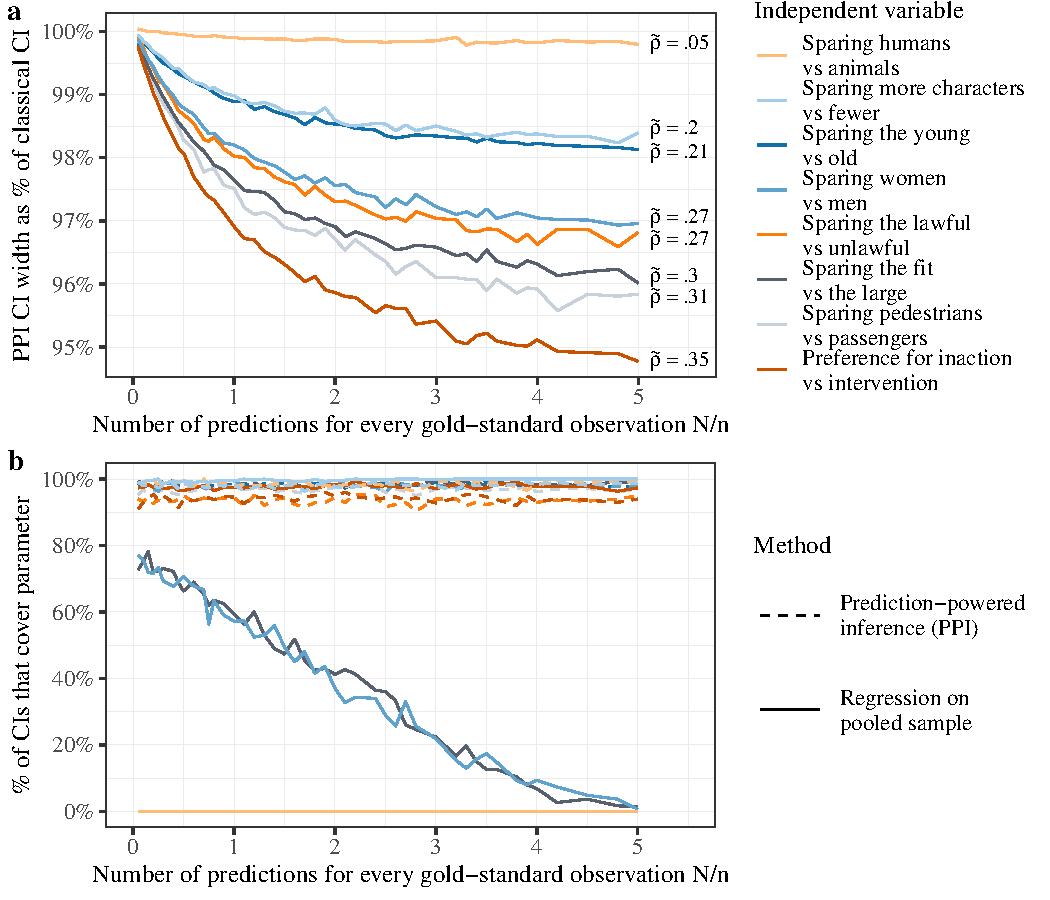
\includegraphics[width=1\linewidth]{8_SimulationResults_gpt4turbo_wp_Saved_Nn_n500.pdf}
    \caption{The x-axes show the ratio of sample sizes $N/n$ with $N$ silicon subjects and $n$ gold standard observations. (\textbf{a}) The y-axis shows the width of the PPI confidence interval (CI) as a share of the CI from a regression on the pooled sample of size $n+N$. Values smaller than $100\%$ indicate the percent reduction in PPI CI width relative to the regression CI (cf. Figure \ref{fig:theo-ppi-classic-ci}). (\textbf{b}) The y-axis shows the percent of CIs calculated with PPI and regression that cover the AMCE estimates from the quota sample of 2,097 Americans; the estimates from this sample are used as the best available approximation of the AMCE parameters.}
    \label{fig:coverage-width}
\end{figure}

\clearpage

Figure \ref{fig:coverage-width} compares statistical precision (i.e., width of confidence intervals) and validity (i.e. percent of confidence intervals that cover the true parameter) in the mixed subjects approach with PPI versus the approach that naively pools human and silicon subjects.
Figure \ref{fig:coverage-width}a shows that adding an increasing number of LLM predictions reduces the width of confidence intervals more strongly for larger values of the PPI correlation $\tilde{\rho}$ (cf. Figure \ref{fig:theo-ppi-classic-ci}).
Figure \ref{fig:coverage-width}b shows that the percent of PPI confidence intervals that cover the parameter remains stable at high levels. In contrast, the coverage of the classical intervals computed for the naive approach remains stable only for some independent variables.
In sum, this analysis illustrates that PPI produces valid point estimates, with increases in statistical precision depending on the 
PPI correlation. The silicon sampling approach may also produce valid point estimates but this is impossible to ascertain without validation on human subjects. PPI automatically handles this validation by introducing a statistical correction to the point estimates derived from LLM predictions.

\section{Conclusion}

Large language models, and generative AI more generally, offer new data sources that may transform the social sciences. Predictions of human behavior---often called ``silicon subjects"---provide a cost-effective and near-instantly available alternative to observing behavior in human subjects studies. However, like novel data sources that have come before \citep{lazer2009css,lazer_computational_2020}, computational social scientists must critically assess the limitations of LLMs and develop robust methods to ensure sound conclusions from this emerging data source. We argue that researchers risk drawing incorrect conclusions when treating LLM predictions as interchangeable with observed human behavior. Estimating parameters based on large numbers of predictions can give a false sense of precision because the confidence intervals will be overly narrow, while the point estimates may systematically diverge from those estimated on a sample of human subjects. Even if LLMs become more accurate in predicting human behavior, these predictions remain of minimal benefit because researchers still need to validate the assumption of interchangeability with an appropriately large sample of human subjects.

We propose that LLM predictions be integrated with, rather than replace, human subjects in what we call a mixed subjects design. We demonstrate and extend prediction-powered inference (PPI), a statistical method that adjusts possibly invalid point estimates derived from LLM predictions to produce valid estimates. Mixed subjects studies with PPI also allow researchers to obtain narrower confidence intervals and higher statistical power than studies with human subjects only. Therefore, the mixed-subjects design with PPI allows researchers to combine the strengths of the human and silicon subjects approach.

Our statistical contributions to PPI are two-fold. First, we derive the PPI correlation $\tilde{\rho}$ as an empirical measure of the extent to which human subjects and LLM predictions are interchangeable. We show that high values of the PPI correlation produce small standard errors for parameters, implying narrower confidence intervals, higher statistical power, and lower costs of conducting mixed subjects experiments relative to human subjects experiments. If LLMs and other algorithms become more capable of predicting human behavior in the future, this improvement will be reflected in higher values for the PPI correlation. More capable algorithms will result in higher statistical precision of PPI estimates and the cost of conducting mixed subjects experiments will further decrease relative to human subjects experiments. 

Our second statistical contribution is a power analysis for PPI that addresses the trade-off between silicon and human subjects if they are not fully interchangeable (i.e., $\tilde{\rho} <1$). The PPI power analysis allows researchers to optimally choose between recruiting \textit{informative but costly} human subjects and \textit{less informative but cheap} silicon subjects. Researchers can allocate a given budget to maximize power or minimize budget expenditure to achieve a desired level of power.  
Statistical software published alongside this article completes the toolkit necessary to conduct mixed subjects studies with PPI.

Our work points to immediate next steps for mixed-subject experimental design. While we leverage PPI to implement these designs, we note that other methods are also well-suited for this purpose. For instance, researchers could combine samples of silicon and human subjects in a Bayesian regression framework (e.g. \citealp{jones2011bayesian}). Here, priors on the parameter values correspond to the degree to which researchers want to treat silicon subjects as interchangeable with human subjects. 
We also want to emphasize that the literature on doubly robust machine learning offers other promising routes for implementing mixed-subjects designs \citep{egami_using_2024-1,kallus_role_2024}. More generally, the development of a robust toolkit of mixed-subject methodologies will allow researchers to leverage LLMs and other forms of generative AI to pursue their research questions.

In a second future direction, the possibility of obtaining valid and precise estimates at low costs from a mixed-subjects design could be leveraged to conduct studies that would otherwise be prohibitively expensive.
For instance, identifying small treatment effects or interactions with sufficient statistical power requires thousands of observations, implying costs that may be too high when estimating these effects with human subjects alone. 
Moreover, studies aimed at systematically exploring a larger number of hypotheses and possible experimental designs have important practical and theoretical implications \citep{almaatooq2024beyond}, but often require an inordinate number of human subjects. The mixed subjects design could be integrated with existing research infrastructure to facilitate such large-scale experiments \citep{almaatouq_empirica_2021}. By reducing the cost of data collection, coupled with valid inferences about parameters, the mixed subjects design could increase scientific productivity and reduce inequality in access to otherwise costly data for research questions and hypotheses. The resulting savings could also be allocated to other research projects or used to pay higher wages to survey participants.

\section*{Data Availability}

A replication package is available at [URL blinded for review].

\newpage
\theendnotes

\newpage
\bibliographystyle{apa}
\bibliography{bibliography.bib}

\begin{appendix}



\captionsetup[figure]{labelformat=simple, labelsep=colon}
\captionsetup[table]{labelformat=simple, labelsep=colon}
\renewcommand{\thefigure}{S\arabic{figure}}
\renewcommand{\thetable}{S\arabic{table}}

\setcounter{figure}{0}
\setcounter{table}{0}

\onehalfspacing
\pagenumbering{arabic}
\setcounter{1}

\section*{\LARGE Supporting Information}



\section{Prediction Powered Inference (PPI)}\label{sec:power}

\subsection{PPI Standard Error and Correlation}\label{sec:ppi-se-and-corr}

In this section, we will define the PPI correlation $\tilde{\rho}$ and show that the standard error of the PPI estimator $\hat{\theta}^{\PPI}$ is equal to 
\begin{equation}\label{eq:PPI-se-supp}
    \mathrm{SE}(\hat{\theta}^{\PPI}) = \frac{\sigma}{\sqrt{n}}\sqrt{1-\frac{N}{N+n}\tilde{\rho}^2}.
\end{equation}
This expression for the standard error is given in equation~\eqref{eq:PPI-se} and used in our power analysis. To define $\tilde{\rho}$ and prove equation~\eqref{eq:PPI-se-supp}, we will use some results and concepts from \cite{angelopoulos2024ppi}. In particular, equation~\eqref{eq:PPI-se-supp} only holds when $\hat{\theta}^{\PPI}$ is the \emph{power-tuned} PPI estimator -- a concept introduced in \cite[Section 6]{angelopoulos2024ppi} and reviewed here.

Let $\{(X_i,Y_i)\}_{i=1}^n$ and $\{\widetilde{X}_i\}_{i=1}^N$ be the labeled and unlabeled datasets as in Section~\ref{sec:PPI}. Let $f$ be the machine learning algorithm that predicts $Y$ from $X$. Let $\ell_\theta(x,y)$ be a loss function with $\theta \in \reals^d$. The loss function $\ell_\theta$ defines an estimand $\theta^\star$ by
\[\theta^\star = \argmin_{\theta \in \reals^d} \mathbb{E}[\ell_\theta(X,Y)]. \]
For example, if $\ell_\theta(x,y) = \frac{1}{2}(x^\top \theta - y)^2$, then $\theta^\star$ is the vector of ordinary least squares coefficients for regressing $Y$ on $X$. 

\cite{angelopoulos2024ppi} introduce a family of estimators $\hat{\theta}^{\PPI}_\lambda$ for $\theta^\star$. These estimators depend on a tuning parameter $\lambda \in \reals$ and are given by
\[
    \hat{\theta}_{\lambda}^\PPI = \argmin_{\theta \in \reals^d}\frac{1}{n}\sum_{i=1}^n \ell_\theta(X_i,Y_i) + \lambda\left(\frac{1}{N}\sum_{i=1}^N \ell_\theta(\widetilde{X}_i,f(\widetilde{X}_i)) - \frac{1}{n}\sum_{i=1}^n \ell_\theta(X_i, f(X_i)\right). 
\]
Taking $\lambda = 0$ corresponds to the classical M-estimator for $\theta^\star$
\[
    \hat{\theta}^{\mathrm{classical}} =\hat{\theta}^\PPI_0 = \argmin_{\theta \in \reals^d} \frac{1}{n}\sum_{i=1}^n \ell_\theta(X_i,Y_i). 
\]
In Theorem~1 of \cite{angelopoulos2024ppi}, the authors show that, under certain assumptions of the loss $\ell_\theta$, the PPI estimator $\hat{\theta}^{\PPI}_\lambda$ satisfies a central limit theorem. Specifically, if $n,N \to \infty$ with $n/N \to r$, then
\begin{equation}
    \label{eq:CLT}   
    \sqrt{n}\left(\hat{\theta}^\PPI_\lambda - \theta^\star\right) \stackrel{d}{\to} \mathcal{N}(0,\Sigma^\lambda),
\end{equation}
where $\mathcal{N}(\mu,\Sigma)$ denoted the $d$-dimensional Guassian distribution with mean $\mu$ and covariance matrix $\Sigma$. The asymptotic covariance matrix $\Sigma^\lambda$ has the following ``sandwich'' form
\begin{align}
    \Sigma^{\lambda} =& H^{-1}_{\theta^\star}\cov(\nabla \ell_{\theta^\star})H^{-1}_{\theta^\star}+\lambda^2(1+r) H^{-1}_{\theta^\star}\cov(\nabla \ell_{\theta^\star}^f )H^{-1}_{\theta^\star}\nonumber \\
    &- \lambda H^{-1}_{\theta^\star}\left(\cov(\nabla \ell_{\theta^\star}^f,\nabla\ell_{\theta^\star})+\cov(\nabla \ell_{\theta^\star},\nabla\ell_{\theta^\star}^f)\right)H^{-1}_{\theta^\star},\label{eq:cov-matrix}
\end{align}
where $\nabla \ell_{\theta^\star}$ is the gradient of $\ell_\theta(X,Y)$ with respect to $\theta$ evaluated at $\theta^\star$, $\nabla \ell_{\theta^\star}^f$ is the gradient of $\ell_\theta(X,f(X))$ evaluated at $\theta^\star$ and $H_\theta^\star = \E[\nabla^2 \ell_{\theta^\star}(X,Y)].$

By equation~\eqref{eq:CLT} the standard error of the $j$th coordinate $\hat{\theta}^{\PPI}_{\lambda,j}$ is $\sqrt{\Sigma^{\lambda}_{j,j}/n}$. We will show that if $\lambda$ is chosen by \emph{power tuning} \citep[Section~6]{angelopoulos2024ppi}, then the PPI standard error will simplify to the expression in \eqref{eq:PPI-se-supp}.

Power tuning \citep[Section~6]{angelopoulos2024ppi} chooses $\lambda$ to minimize $\Sigma_{j,j}^\lambda$. This is equivalent to choose $\lambda$ to minimize the standard error of $\hat{\theta}^{\PPI}_{\lambda,j}$. From \eqref{eq:cov-matrix}, we have
\begin{align*}
    \Sigma^{\lambda}_{j,j} &= \left[H^{-1}_{\theta^\star}\cov(\nabla \ell_{\theta^\star})H^{-1}_{\theta^\star}\right]_{j,j}+\lambda^2(1+r) \left[H^{-1}_{\theta^\star}\cov(\nabla \ell_{\theta^\star}^f )H^{-1}_{\theta^\star}\right]_{j,j} \\
    &- \lambda \left[H^{-1}_{\theta^\star}\left(\cov(\nabla \ell_{\theta^\star}^f,\nabla\ell_{\theta^\star})+\cov(\nabla \ell_{\theta^\star},\nabla\ell_{\theta^\star}^f)\right)H^{-1}_{\theta^\star}\right]_{j,j}\\
    &=\left[H^{-1}_{\theta^\star}\cov(\nabla \ell_{\theta^\star})H^{-1}_{\theta^\star}\right]_{j,j}
    +\lambda^2 (1+r) \left[H^{-1}_{\theta^\star}\cov(\nabla \ell_{\theta^\star}^f)H^{-1}_{\theta^\star}\right]_{j,j}\\
    &- 2\lambda \left[H^{-1}_{\theta^\star}\cov(\nabla \ell_{\theta^\star}^f,\nabla\ell_{\theta^\star})H^{-1}_{\theta^\star}\right]_{j,j}.
\end{align*}
To get the final expression, we have used that $\cov(\nabla \ell_{\theta^\star}^f,\nabla \ell_{\theta^\star})^\top = \cov(\nabla \ell_{\theta^\star},\nabla \ell_{\theta^\star}^f)$ and that $H_{\theta^*}^{-1}$ is symmetric. The function $\lambda \mapsto \Sigma_{j,j}^\lambda$ is quadratic in $\lambda$ and its minimum occurs at
\[
    \lambda^\star_j = \frac{1}{1+r}\frac{\left[H^{-1}_{\theta^\star}\cov(\nabla \ell_{\theta^\star}^f,\nabla\ell_{\theta^\star})H^{-1}_{\theta^\star}\right]_{j,j}}{\left[H^{-1}_{\theta^\star}\cov(\nabla \ell_{\theta^\star}^f)H^{-1}_{\theta^\star}\right]_{j,j}}. 
\]
Furthermore, when $\lambda = \lambda^\star_{j}$, we have
\begin{align*}
    \Sigma^{\lambda^\star_j}_{j,j} =&  \left[H^{-1}_{\theta^\star}\cov(\nabla \ell_{\theta^\star})H^{-1}_{\theta^\star}\right]_{j,j}\\
    &\times \left( 1 - \frac{1}{1+r}\frac{\left[H^{-1}_{\theta^\star}\cov(\nabla \ell_{\theta^\star}^f,\nabla\ell_{\theta^\star})H^{-1}_{\theta^\star}\right]_{j,j}^2}{\left[H^{-1}_{\theta^\star}\cov(\nabla \ell_{\theta^\star}^f)H^{-1}_{\theta^\star}\right]_{j,j}\left[H^{-1}_{\theta^\star}\cov(\nabla \ell_{\theta^\star})H^{-1}_{\theta^\star}\right]_{j,j}}\right) \\
    =&\sigma^2_j\left(1-\frac{1}{1+r}\tilde{\rho}^2_j\right),
\end{align*}
where we have defined $\sigma^2_j = \left[H^{-1}_{\theta^\star}\cov(\nabla \ell_{\theta^\star})H^{-1}_{\theta^\star}\right]_{j,j}$ and
\begin{equation}\label{eq:PPI_corr}
    \tilde{\rho}^2_j =   \frac{\left[H^{-1}_{\theta^\star}\cov(\nabla \ell_{\theta^\star}^f,\nabla\ell_{\theta^\star})H^{-1}_{\theta^\star}\right]_{j,j}^2}{\left[H^{-1}_{\theta^\star}\cov(\nabla \ell_{\theta^\star}^f)H^{-1}_{\theta^\star}\right]_{j,j}\left[H^{-1}_{\theta^\star}\cov(\nabla \ell_{\theta^\star})H^{-1}_{\theta^\star}\right]_{j,j}}.
\end{equation}
The quantity $\sigma_j^2$ is the asymptotic variance of the classical estimator $\hat{\theta}^{\mathrm{classical}}$ and $\tilde{\rho}_j$ is the PPI correlation. 

Since $r=\frac{n}{N}$, the standard error of $\hat{\theta}^{\PPI}_{\lambda^\star_j,j}$ from a sample of $n$ labeled data points and $N$ unlabeled data point is
\[
   \mathrm{SE}(\hat{\theta}^{\PPI}_{\lambda^\star_j, j})= \sqrt{\Sigma_{j,j}^{\lambda^\star_j}/n} = \frac{\sigma_j}{\sqrt{n}}\sqrt{1-\frac{N}{N+n}\tilde{\rho}^2_j}.  
\]
In practice, $\lambda^\star_j$ has to be estimated. \cite{angelopoulos2024ppi} provide a consistent estimator $\hat{\lambda}_j$ for $\lambda^\star_j$ and show that $\hat{\theta}_{\hat{\lambda}_j,j}^{\PPI}$ achieves the same asymptotic variance as $\hat{\theta}^{\PPI}_{\lambda^\star_j,j}$. 

To simplify notation, we will write $\hat{\theta}^{\PPI}$ for $\hat{\theta}^{\PPI}_{\hat{\lambda}_j,j}$ and $\sigma$ instead of $\sigma_j$ and $\tilde{\rho}$ instead of $\tilde{\rho}_j$. With this notation we have
\[ 
    \mathrm{SE}(\hat{\theta}^{\PPI}) = \frac{\sigma}{\sqrt{n}}\sqrt{1-\frac{N}{N+n}\tilde{\rho}^2},
\]
as claimed in equations~\eqref{eq:PPI-se} and \eqref{eq:PPI-se-supp}.

\subsection{The Effective Sample Size in PPI}\label{sec:effective-sample-size}

The \emph{effective sample size} is the number $n_0$ of labeled data points that would give the same standard error of using PPI with $n$ labeled points and $N$ unlabeled points. The standard error with $n_0$ labeled data points is simple $\sigma/\sqrt{n_0}$. Equating this with the PPI standard error in \eqref{eq:PPI-se-supp} gives
\[
    n_0 = n \cdot \frac{n+N}{n+N-N\tilde{\rho}^2}. 
\]
Let $k = \frac{N}{n}$. Then, the effective sample size in PPI increases the number of human subjects by a factor of 
\[ 
    \frac{1+k}{1+k-k\tilde{\rho}^2} \ge 1.
\]
When $\tilde{\rho}^2=1$, this factor equals $1+k$ and the effective sample size is $n(1+N/n)=n+N$. That is, the effective sample size is the size of the full pooled sample. When $\tilde{\rho}=0$, this factor equals $1$ and the effective sample size is $n$ meaning that only the labeled samples are used.


\subsection{The Cost of PPI and Classical Inference}

In this section we derive the percentage of cost saved by PPI as reported in Figure~\ref{fig:perc-cost-reduction}. This is done by first finding all pairs of sample sizes $(n,N)$ that achieve the same standard error as a baseline classical experiment with $n_0$ labeled data points. Then, given the costs of collecting a labeled and unlabeled sample, we find the optimal pair $(n^\star,  N^\star)$ that minimizes the cost of PPI while still having the same power as the baseline classical experiment. The results in this section are used in the next two sections to derive the cheapest pair and most powerful pair for our power analysis.

Let $S(n,N)$ be the standard error of the PPI estimate, so that
\[
    S(n,N) = \frac{\sigma}{\sqrt{n}}\sqrt{1- \frac{N}{N+n}\tilde{\rho}^2}. 
\]
In a baseline experiment $n_0$ labeled samples, the standard error is $S(n_0, 0) = \sigma/\sqrt{n_0}$. By rearranging the equation $S(n,N) = \sigma/\sqrt{n_0}$, it can be shown that $S(n,N)=\sigma/\sqrt{n_0}$ if and only if 
\begin{equation}
n_0(1-\tilde{\rho}^2) < n \le n_0 \quad \text{and} \quad
    N = \frac{n(n_0 - n)}{n-n_0(1-\tilde{\rho}^2)} .\label{eq:level curves}
\end{equation}
Let $c_X$ and $c_Y$ be the cost of collecting $X$ and $Y$ and let $c_f$ be the cost of computing $f(X)$.  The cost of performing PPI with $n$ labeled subjects and $N$ unlabeled subjects is 
\begin{equation*}
    C(n,N) = (c_X+c_Y+c_f)n + (c_X+c_f)N.
\end{equation*}
This is because PPI requires $X_i$, $Y_i$, and $f(X_i)$ for the $n$ labeled samples and requires $\widetilde{X}_i$ and $f(\widetilde{X}_i)$ for the $N$ unlabeled samples. If we let $\gamma = (c_X+c_f)/c_Y$, then
\begin{equation*}
    C(n,N) = c_Y((1+\gamma) n + \gamma N)
\end{equation*}


Our goal is to find the pair $(n^\star, N^\star)$ that satisfies the constraints in equation~\eqref{eq:level curves} and minimizes $C(n,N)$. That is, $(n^\star, N^\star)$ is the solution to the optimization problem
\begin{equation}
\begin{array}{ll}
        \mbox{minimize} & C(n,N)\\
        \mbox{subject to} & \mbox{equation }\eqref{eq:level curves}
    \end{array}
\end{equation}
This optimization problem can be solved by first substituting $N=\frac{n(n_0-n)}{n-n_0(1-\tilde{\rho}^2)}$ into $C(n,N)$. This gives the cost as a function of $n$ alone. Setting the derivative of this function equal to zero gives
\begin{equation}\label{eq:nstar}
    n^\star = n_0\left(1-\tilde{\rho}^2+\sqrt{\gamma \tilde{\rho}^2(1-\tilde{\rho}^2)}\right)\quad \text{and} \quad N^\star =   \frac{n^\star(n_0-n^\star)}{n^\star - (1-\tilde{\rho}^2)n_0}.
\end{equation}
At the optimal pair $(n^\star, N^\star)$, the cost is 
\begin{equation}\label{eq:best-cost}
    C(n^\star, N^\star) = c_Y n_0\left(1-\tilde{\rho}^2 + \gamma\tilde{\rho}^2 +2\sqrt{\gamma \tilde{\rho}^2(1-\tilde{\rho}^2)} \right). 
\end{equation}
In contrast, the cost of performing classical inference with $n_0$ human subjects is 
\[
    C_0(n_0) = (c_Y+c_X)n_0. 
\]
This equation for the costs in classical inference is simpler since we do not need to compute $f(X_i)$ on the labeled data. It follows that PPI is more cost-effective than classical inference if and only if 
\[
c_Y \left(1-\tilde{\rho}^2 + \gamma\tilde{\rho}^2 +2\sqrt{\gamma \tilde{\rho}^2(1-\tilde{\rho}^2)} \right) \le c_Y+c_X.
\]
Furthermore, when this condition is satisfied, the optimal \emph{absolute} cost savings from PPI are
\[
C_0(n_0) - C(n^\star, N^\star) = n_0(c_X + c_Y(\tilde{\rho}^2 - \gamma \tilde{\rho}^2 - 2 \sqrt{\gamma \tilde{\rho}^2 (1-\tilde{\rho}^2)})).
\]
The \emph{relative} cost savings from PPI are 
\[
\frac{C_0(n_0)-C(n^\star, N^\star)}{C_0(n_0)} = \frac{c_X}{c_Y} + \tilde{\rho}^2 - \gamma \tilde{\rho}^2 - 2 \sqrt{\gamma \tilde{\rho}^2(1-\tilde{\rho}^2)}.
\]
In the context of mixed subjects experiments, it is natural to take $c_X=0$. This is because $c_X$ is simply the cost of recording demographic information or treatment assignments which is small compared to the cost of the full survey. When $c_X=0$, we have $\gamma = c_f/c_Y$ and PPI is strictly more cost efficient than classical inference if and only if 
\[
\tilde{\rho}^2 - \gamma\tilde{\rho}^2 -2\sqrt{\gamma \tilde{\rho}^2(1-\tilde{\rho}^2)} > 0.
\]
This is equivalent to
\[
\tilde{\rho}^2 > \frac{4 \gamma}{(1+\gamma)^2}.
\]
That is, the PPI correlation must be sufficiently high compared to the relative cost of collecting a labeled or unlabeled sample. When this condition is met, the expressions for the absolute and relative cost reductions simplify and become
\begin{align}
    C_0(n_0)-C(n^\star, N^\star) &= n_0c_Y(\tilde{\rho}^2 - \gamma \tilde{\rho}^2 - 2 \sqrt{\gamma \tilde{\rho}^2 (1-\tilde{\rho}^2)},\nonumber \\
    \frac{C_0(n_0)-C(n^\star, N^\star)}{C_0(n_0)}& =  \tilde{\rho}^2 - \gamma \tilde{\rho}^2 - 2 \sqrt{\gamma \tilde{\rho}^2(1-\tilde{\rho}^2)}.\nonumber
\end{align}
Furthermore, the ratio of $C(n^\star,N^\star)$ over $C_0(n_0)$ simplifies to 
\begin{equation}
    \frac{C(n^\star, N^\star)}{C_0(n_0)} = 1 - \tilde{\rho} +\gamma \tilde{\rho}+2\sqrt{\gamma \tilde{\rho}^2(1-\tilde{\rho}^2)}. \label{eq:percent_cost}
\end{equation}
The curves in Figure~\ref{fig:perc-cost-reduction} plot equation~\eqref{eq:percent_cost} as a function of $1/\gamma=c_Y/c_f$ for different values of $\tilde{\rho}$.

\subsection{Power Analysis for the Most Powerful Pair}\label{sec:most-powerful-pair}

The power analysis for the most powerful pair identifies the pair of sample sizes $(n^\star, N^\star)$ the achieves the smallest standard error subject to a budget constraint. Once the most powerful pair has been computed, the standard error of the PPI estimate can be approximated. Likewise, we can estimate the power of a PPI hypothesis test that uses $(n^\star, N^\star)$.

The inputs required to compute the most powerful pair are the PPI correlation $\tilde{\rho}$, the costs $c_Y, c_f, c_X$ defined above, and a budget $B$. The PPI correlation would be estimated from data and the costs and budget must be specified by the user. Once these inputs have been provided, $\gamma = (c_X+c_f)/c_Y$ can be computed. 

The previous section determined when classical inference was more cost-effective than PPI. When classical inference is more cost-effective, the most powerful pair results from spending all the budget on labeled samples and using no unlabeled samples. Therefore, if 
\[
    c_Y \left(1-\tilde{\rho}^2 + \gamma\tilde{\rho}^2 +2\sqrt{\gamma \tilde{\rho}^2(1-\tilde{\rho}^2)} \right) > c_Y+c_X,
\] then
\[
    n^\star = \frac{B}{c_X+c_Y}\quad \text{and} \quad N^\star = 0. 
\]
If PPI is more cost-effective than classical inference, then the budget should be allocated so that $C(n^\star, N^\star) = B$ where $n^\star, N^\star$ and $C(n^\star,N^\star)$ are as in equations~\eqref{eq:nstar} and \eqref{eq:best-cost}. This means that if 
\[
    c_Y \left(1-\tilde{\rho}^2 + \gamma\tilde{\rho}^2 +2\sqrt{\gamma \tilde{\rho}^2(1-\tilde{\rho}^2)} \right) \le c_Y+c_X,
\] then 
\[
     n^\star = n_0\left(1-\tilde{\rho}^2+\sqrt{\gamma \tilde{\rho}^2(1-\tilde{\rho}^2)}\right)\quad \text{and} \quad N^\star =   \frac{n^\star(n_0-n^\star)}{n^\star - (1-\tilde{\rho}^2)n_0},
\]
where 
\[
    n_0 = \frac{B}{c_Y\left(1-\tilde{\rho}^2 + \gamma\tilde{\rho}^2 +2\sqrt{\gamma \tilde{\rho}^2(1-\tilde{\rho}^2)} \right)}.
\]
Once the most powerful pair $(n^\star, N^\star)$ has been computed, the standard error of the PPI estimate from using $(n^\star, N^\star)$ and the power of using $(n^\star, N^\star)$ can also be approximated. The dataset used to estimate $\tilde{\rho}$ can also be used to estimate $\sigma$. Given $\sigma$, the standard error of $\hat{\theta}^{\PPI}$ when using $(n^\star, N^\star)$ is
$S(n^\star,N^\star) = \frac{\sigma}{\sqrt{n^\star}}\sqrt{1-\frac{N^\star}{N^\star+n^\star}\tilde{\rho}^2}$. 

To estimate the power of testing the null hypothesis $\theta = \theta_0$, we can use the supplied dataset to estimate an effect size $\delta = \hat{\theta}^{\PPI}-\theta_0$. The power of using $(n^\star, N^\star)$ in a level $\alpha$ test of the hypothesis $\theta = \theta_0$ is 
\begin{equation}\label{eq:power}
1-\beta = 1 - \Phi\left(z_{1-\alpha/2} - \frac{\delta}{S(n^\star,N^\star)}\right) + \Phi\left(-z_{1-\alpha/2}-\frac{\delta}{S(n^\star,N^\star)}\right),
\end{equation}
where $\Phi$ is the cumulative distribution function of the standard normal distribution and $z_{p}$ is the $p$th quantile of the standard normal distribution.

\subsection{Power Analysis for the Cheapest Pair}\label{sec:cheapest-pair}

The power analysis for the cheapest pair identifies a pair of sample sizes $(n^\star, N^\star)$ such that achieves a desired standard error of size at most $\varepsilon$. Once the cheapest pair has been computed, the cost of the experiment can be calculated.

The inputs required to compute the cheapest pair are the PPI correlation $\tilde{\rho}$, the standard deviation of the classical estimator $\sigma$, the costs $c_Y,c_f,c_X$ and the desired standard error $\varepsilon > 0$. As before, the parameters $\tilde{\rho}$  and $\sigma$ are estimated from a dataset and $c_Y,c_f,c_X$ and $\varepsilon$ are provided by the user. Again, set $\gamma = (c_X+c_f)/c_Y$.

When classical inference is more cost-effective than PPI, the cheapest pair will use only labeled samples. This means that if
\[
   c_Y \left(1-\tilde{\rho}^2 + \gamma\tilde{\rho}^2 +2\sqrt{\gamma \tilde{\rho}^2(1-\tilde{\rho}^2)} \right) > c_Y+c_X,
\]
then
\[ 
    n^\star = \frac{\sigma^2}{\varepsilon^2} \quad \text{and} \quad N^\star = 0.
\]
When PPI is more cost-effective than classical inference, then $(N^\star, n^\star)$ should be chosen so that $S(n^\star, N^\star) = \varepsilon$ where $n^\star$ and $N^\star$ are as in equation~\eqref{eq:nstar} and hence $S(n^\star, N^\star) = \frac{\sigma}{\sqrt{n_0}}$. Thus, if
\[
    c_Y \left(1-\tilde{\rho}^2 + \gamma\tilde{\rho}^2 +2\sqrt{\gamma \tilde{\rho}^2(1-\tilde{\rho}^2)} \right) \le c_Y+c_X,
\] then 
\[
     n^\star = n_0\left(1-\tilde{\rho}^2+\sqrt{\gamma \tilde{\rho}^2(1-\tilde{\rho}^2)}\right)\quad \text{and} \quad N^\star =   \frac{n^\star(n_0-n^\star)}{n^\star - (1-\tilde{\rho}^2)n_0},
\]
where 
\[
    n_0 = \frac{\sigma^2}{\varepsilon^2}.
\]
Once $(n^\star, N^\star)$ have been computed, the cost of $(n^\star, N^\star)$ can be computed. The cost varies depending on whether classical inference or PPI was used. When classical inference is used, the cost is
\[ 
    C_0(n^\star) = (c_Y+c_X)n^\star.
\]
When PPI is used, the cost is
\[
    C(n^\star, N^\star) = (c_Y+c_X+c_f)n^\star + (c_X+c_f)N^\star.
\]
The user may wish to provide a level of power, $1-\beta$, instead of a desired standard error $\varepsilon$. To compute the cheapest pair in this setting, the user must provide or estimate the difference in the alternative and null parameters $\delta=\theta_{H_a}-\theta_{H_0}$. The user must also provide a level of the test $\alpha$. Once these have been provided, the desired standard error $\varepsilon>0$ is the solution to the equation
\[
1-\beta = 1 - \Phi\left(z_{1-\alpha/2} - \frac{\delta}{\varepsilon}\right) + \Phi\left(-z_{1-\alpha/2}-\frac{\delta}{\varepsilon}\right),
\]
where $\Phi$ and $z_p$ are as in equation~\eqref{eq:power}. Once $\varepsilon$ is known, the power analysis for the cheapest pair proceeds as above.

% \subsection{Minimum cost PPI}

% PPI can achieve the same level of statistical precision as classical inference while using fewer observations from human subjects \citep{angelopoulos2024ppi}. Below we quantify this increase in precision and how to choose 

% Let $S(n,N)$ be the PPI standard error for the estimate $\hat{\theta}^{\PPI}$ when using $n$ human samples and $N$ silicon samples. That is,
% \[ 
%     S(n,N) = \frac{\sigma}{\sqrt{n}}\sqrt{1-\frac{N}{n+N}\tilde{\rho}^2}.
% \]
% To quantify the increase in statistical precision in PPI relative to classical inference, let $n_0$ be a baseline sample size of an experiment with only human subjects. The standard error of using $n_0$ human subjects and no silicon subject is 
% \[
%     S(n_0,0) = \frac{\sigma}{\sqrt{n_0}}. 
% \]
% For any $n$ satisfying $n_0(1-\tilde{\rho}^2) < n \le n_0$, if $N=\frac{n(n-n_0)}{n-n_0(1-\tilde{\rho}^2)}$, then 
% \[
%     S(n,N)=S(n_0,0).
% \]
% Equivalently, the level curves of the function $S(n,N)$ are given by
% \begin{equation}
%     N = \frac{n(n_0 - n)}{n-n_0(1-\tilde{\rho}^2)}, \quad n_0(1-\tilde{\rho}^2) < n \le n_0.\label{eq:level curves}
% \end{equation}

% There are three distinct costs involved in performing PPI: the cost $c_X$ of collecting an unlabeled sample $X$, the cost $c_Y$ of collecting the label $Y$, and the cost $c_f$ of running the prediction algorithm to compute $f(X)$. For a pair of sample sizes $(n,N)$, the total cost is
% \[
%     c(n,N) = c_X(n+N) + c_Yn + c_f(n+N) = c_Yn + (c_X+c_f)(n+N). 
% \]
% In a mixed subject experiment, we will assume that $c_X = 0$.
%  That is, the cost of human subject is exactly equal to $c_Y$ and the cost of prompting the LLM is $c_f$. Typically, we will also have $c_f \ll c_Y$. That is, the cost of collecting human responses $Y$ far outweighs the cost of generating a silicon sample $f(X)$.

% Let $\gamma = \frac{c_f}{c_Y}$ be the ratio of the cost of a silicon subjects to the cost of a human subjects. Then, the cost of performing PPI in a mixed subject experiment is
% \begin{equation}
%     c(n,N) = c_Y\left(n + \gamma (n+N)\right). \label{eq:cost}
% \end{equation}
% This is because we must prompt the LLM for every human subject and every silicon subject.

% By substituting \eqref{eq:level curves} into \eqref{eq:cost}, we can  minimize over $n$ to identify the most cost-effective way of using PPI to obtain a point estimate with a standard error of size $\sigma/\sqrt{n_0}$. i.e., a level statistical precision on par with classical inference with $n_0$ human subjects. 

% The minimum cost occurs at
% \begin{equation}\label{eq:nstar}
%     n^\star = n_0\left(1-\tilde{\rho}^2+\sqrt{\gamma \tilde{\rho}^2(1-\tilde{\rho}^2)}\right), \quad N^\star = n^\star\cdot  \frac{n_0-n^\star}{n^\star - (1-\tilde{\rho}^2)n_0}.
% \end{equation}
% The minimal cost of using the sample size $(n^\star,N^\star)$ is
% \begin{equation}\label{eq:best-cost}
%     c(n^\star, N^\star) = c_Y n_0\left(1-\tilde{\rho}^2 + \gamma\tilde{\rho}^2 +2\sqrt{\gamma \tilde{\rho}^2(1-\tilde{\rho}^2)} \right). 
% \end{equation}
% The cost of performing classical inference is simply $c_Y n_0$. Thus, PPI is more cost-effective than classical inference when  $\tilde{\rho}^2 - \gamma\tilde{\rho}^2 -2\sqrt{\gamma \tilde{\rho}^2(1-\tilde{\rho}^2)} >0$. This is equivalent to
% \[
%     \tilde{\rho} > \frac{2\sqrt{\gamma}}{1+\gamma}.
% \]
% That is, the correlation $\tilde{\rho}$ must be larger than $2\sqrt{\gamma}/(1+\gamma)$ to improve precision over classic inference. Beyond this minimal condition, we can quantify the cost reduction when using PPI. The \textit{absolute} cost reduction of PPI at the optimal budget $(n^\star,N^\star)$ compared to classical inference are
% \[
%     c_Yn_0-c(n^\star,N^\star) = c_Yn_0\left(\tilde{\rho}^2 - \gamma\tilde{\rho}^2 -2\sqrt{\gamma \tilde{\rho}^2(1-\tilde{\rho}^2)}\right).
% \]
% The \textit{percent} cost reduction of PPI using the optimal sample sizes is thus
% \[ 
%     \frac{c_Yn_0-c(n^\star,N^\star)}{c(n^\star,N^\star)} = \tilde{\rho}^2 - \gamma\tilde{\rho}^2 -2\sqrt{\gamma \tilde{\rho}^2(1-\tilde{\rho}^2)}.
% \]
% For example, we could take $c_Y = \$3.20$ which corresponds to paying respondents a California minimum wage for filling out a 12 minute survey. If we let $c_f= 0.003$ be the cost of simulating a survey session, we have $\gamma = \frac{0.003}{3.20}=0.0009375$. Thus, for PPI to outperform classical inference, it is necessary that 
% \[
%     \tilde{\rho} > \frac{2\sqrt{0.0009375}}{1+0.0009375} \approx 0.061.
% \]
% In the moral machine dataset, the largest value of $\tilde{\rho}$ was $0.35$. For this value, $\tilde{\rho}$, the savings are approximately $0.102\cdot c_Yn_0$, so that PPI can save $10.2\%$ of the costs compared to classical inference.

\section{Details on the Moral Machine Experiment}\label{sec:appendix-moral-machine}


\subsection{Example of a Moral Dilemma}


\begin{figure}[H]
    \centering
    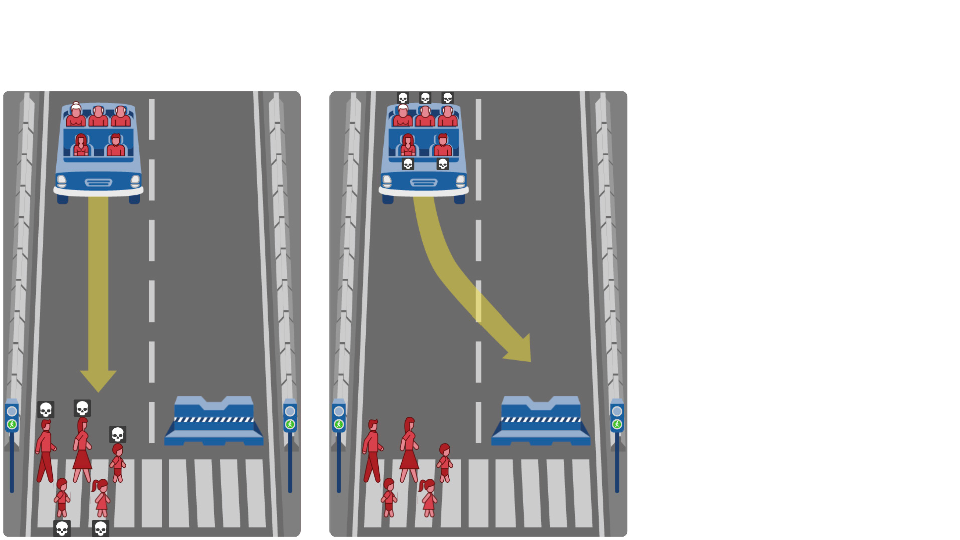
\includegraphics[width=0.85\linewidth]{EH3SfatQP3hygSpzF.pdf}
    \caption{Example dilemma presented to a survey respondent in the Moral Machine Experiment. The image was created on the \textit{moralmachine.net} website with information from the replication data for \citet{awad_moral_2018}.}
    \label{fig:moral-dilemma}
\end{figure}

\newpage

\subsection{Example Prompt}

The LLM was given the following prompt to predict the survey respondent's decision to the moral dilemma. The order of the demographic information was randomized.

\tcbset{
    colback=gray!10,
    colframe=white,
    width=\textwidth,
    enlarge left by=0cm,
    boxrule=0pt,
    round corners,
    left=1cm,
    right=1cm,
    top=0.5cm,
    bottom=0.5cm
}

\begin{tcolorbox}
Carefully consider the following information and think step by step. You are an American with the following characteristics:  
\vspace{5pt}

\begin{itemize}[noitemsep]
    \item You earn an annual income of under \$5,000 US dollars.
    \item Your highest level of education is a high school diploma.
    \item You are 35 years old.
    \item You are a man.
    \item On a scale from 0 (Not Religious) to 100 (Very Religious), you report a score of 0 for your religious views.
    \item On a scale from 0 (Conservative) to 100 (Progressive), you report a score of 100 for your political views.
\end{itemize}

\vspace{5pt}
Consider that pedestrians are crossing a zebra crossing that spans two lanes. Please indicate which case is better for autonomous driving by choosing either `Case 1' or `Case 2'. Respond with one word only. 
\vspace{5pt}

Case 1. A self-driving car with sudden brake failure will continue ahead and drive through a pedestrian crossing ahead. This will result in the death of 1 man, 1 girl, 2 boys, and 1 woman, who were abiding by the law by crossing on the green signal. Meanwhile, it will spare 1 man, 1 elderly woman, 2 elderly men, and 1 woman, who were inside the car.
\vspace{5pt}

Case 2. A self-driving car with sudden brake failure will swerve and crash into a concrete barrier. This will result in the death of 1 man, 1 elderly woman, 2 elderly men, and 1 woman, who were inside the car. Meanwhile, it will spare 1 man, 1 girl, 2 boys, and 1 woman, who were abiding by the law by crossing on the green signal.

\end{tcolorbox}

\subsection{Summary Statistics on Sampling}


\begin{figure}[H]
    \centering
    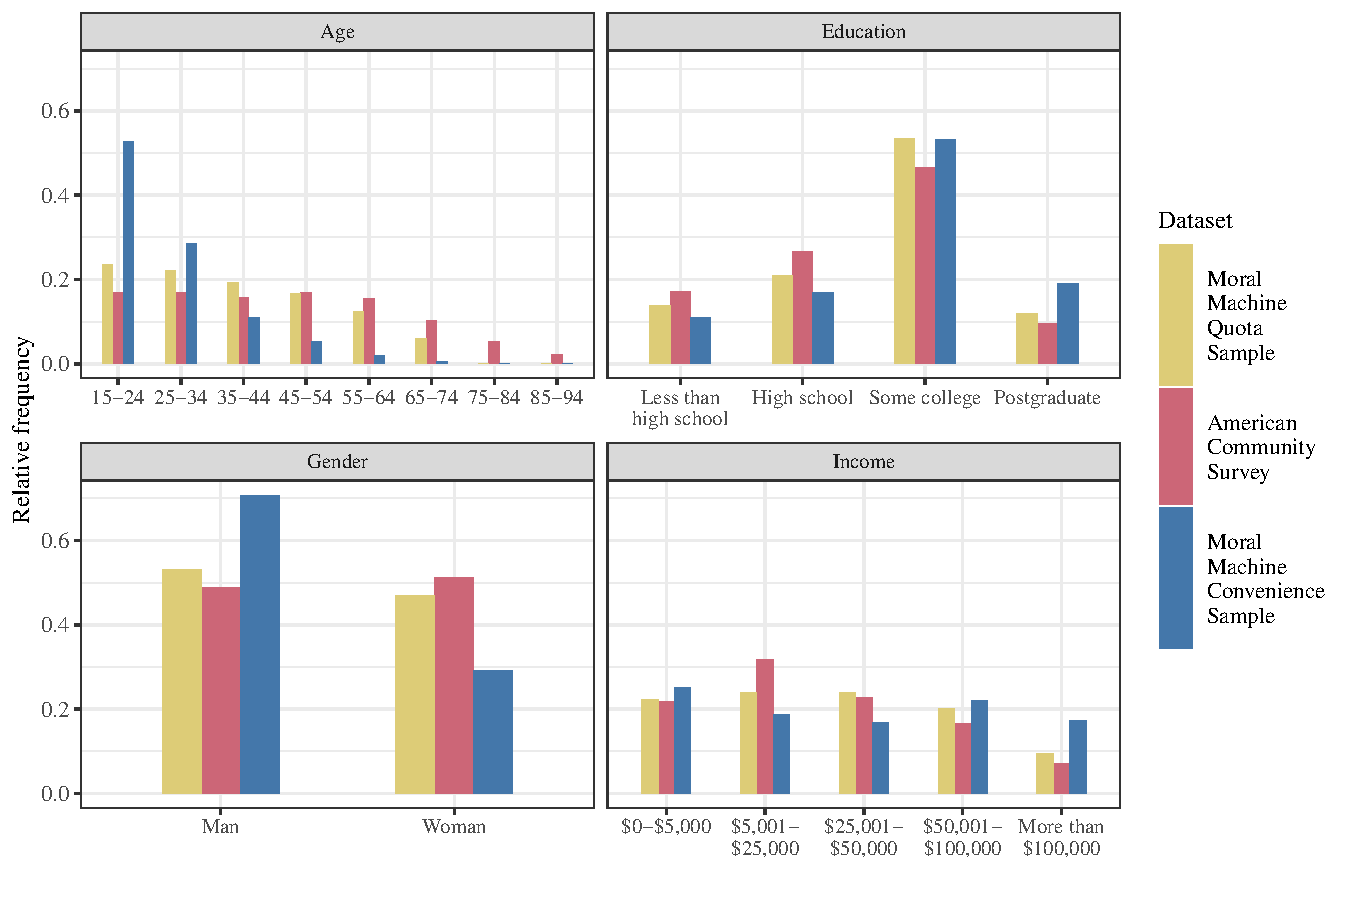
\includegraphics[width=1\linewidth]{2_DemographicDistribution.pdf}
    \caption{Comparison of demographic distributions of the convenience sample reported in the Moral Machine Experiment, the 2016 American Community Survey, and the random sample from the Moral Machine Experiment with quotas from the American Community Survey.}
    \label{fig:demographic-distribution}
\end{figure}

\newpage

\subsection{Replication of AMCE Estimates}

Figure \ref{fig:amce-estimates} compares the estimated causal effects of scenario attributes on the decision to save characters across samples. Compared to the quota sample of Americans from the Moral Machine experiment (yellow), the LLMs often fail to accurately predict how survey respondents' decisions depend on the scenario's characteristics (blue). 

For completeness, we also show the estimated AMCEs reported in \citet{awad_moral_2018}. Although their estimates are based on a cross-country convenience sample and are not expected to align perfectly with those from the quota sample of Americans, the differences are generally small.
\vspace{10pt}

\begin{figure}[H]
    \centering
    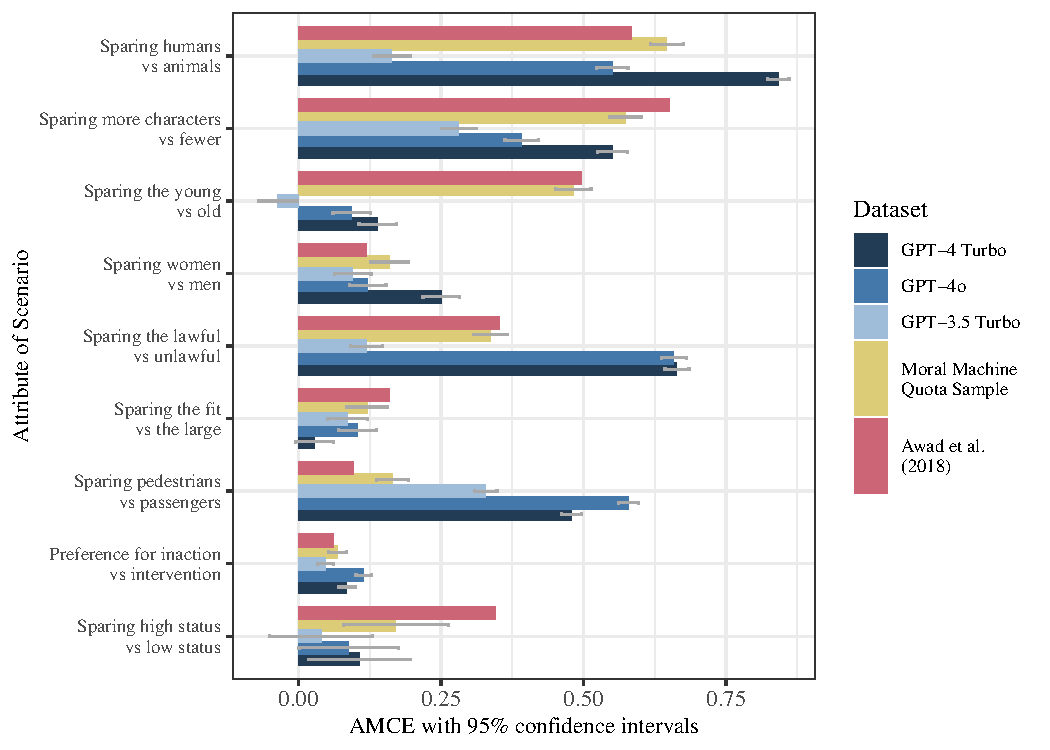
\includegraphics[width=1\linewidth]{8_AMCEs.pdf}
    \caption{Comparison of AMCE estimates from human subjects against silicon subjects. Note that \citet{awad_moral_2018} do not report confidence intervals due to their negligible width, a consequence of the large sample size.}
    \label{fig:amce-estimates}
    \vspace{0.5cm}
\end{figure}


\newpage
\subsection{Prompting LLMs to Predict Decisions to Moral Dilemmas}\label{sec:prompt-llms}

\vspace{10pt}
\begin{table}[H]
\begin{center}
    
\begin{tabular}{|l|l|l|l|l|l|}
\hline
\textbf{\begin{tabular}[c]{@{}l@{}}Language\\ model\end{tabular}} &
  \textbf{\begin{tabular}[c]{@{}l@{}}Context\\ window\end{tabular}} &
  \textbf{\begin{tabular}[c]{@{}l@{}}Training\\ data\end{tabular}} &
  \textbf{\begin{tabular}[c]{@{}l@{}}Input cost\\ 1K tokens\end{tabular}} &
  \textbf{\begin{tabular}[c]{@{}l@{}}Output cost\\ 1K tokens\end{tabular}} \\ \hline
gpt-4-turbo        & 128,000 tokens & Up to Dec 2023 & \$0.010  & \$0.030  \\ \hline
gpt-4o             & 128,000 tokens & Up to Oct 2023 & \$0.005  & \$0.015  \\ \hline
gpt-3.5-turbo-0125 & 16,385 tokens  & Up to Sep 2021 & \$0.0005 & \$0.0015 \\ \hline
\end{tabular}
\caption{Details on LLMs used to predict survey responses}
\label{tab:model-overview}
\end{center}
\end{table}


\vspace{2cm}

\renewcommand{\arraystretch}{0.9}
\begin{table}[!h]
\centering
\begin{tabular}[t]{llcc}
\toprule
Model & Type & Correlation & N\\
\midrule
 & Prediction & 0.361 & 22315\\
\cmidrule{2-4}
 & Replicate 1 & 0.346 & 5000\\
\cmidrule{2-4}
 & Replicate 2 & 0.344 & 5000\\
\cmidrule{2-4}
 & Mode across prediction and replicates & 0.347 & 5000\\
\cmidrule{2-4}
\multirow{-5}{*}{\raggedright\arraybackslash GPT4 Turbo} & Without persona & 0.337 & 4989\\
\cmidrule{1-4}
 & Prediction & 0.311 & 22312\\
\cmidrule{2-4}
 & Replicate 1 & 0.325 & 5000\\
\cmidrule{2-4}
 & Replicate 2 & 0.304 & 5000\\
\cmidrule{2-4}
 & Mode across prediction and replicates & 0.317 & 5000\\
\cmidrule{2-4}
\multirow{-5}{*}{\raggedright\arraybackslash GPT4o} & Without persona & 0.293 & 4974\\
\cmidrule{1-4}
 & Prediction & 0.113 & 22314\\
\cmidrule{2-4}
 & Replicate 1 & 0.112 & 4999\\
\cmidrule{2-4}
 & Replicate 2 & 0.129 & 4999\\
\cmidrule{2-4}
 & Mode across prediction and replicates & 0.144 & 4998\\
\cmidrule{2-4}
\multirow{-5}{*}{\raggedright\arraybackslash GPT3.5 Turbo} & Without persona & 0.174 & 5000\\
\bottomrule
\end{tabular}
\caption{\label{tab:corr-tab}Pearson correlation of survey respondents' decision for a moral dilemma with the LLM predicted decision. In addition to the 22,315 predictions, we assess how the correlation varies by prompting the LLM to give 5,000 additional predictions. We form a composite from the modal prediction of three identical prompts. For a separate set of predictions, we omit the demographic persona from the prompt.}
\end{table}

\newpage 
\section{Example Power Analysis}\label{sec:gpower}

We used G*Power, a software by \citet{faul_statistical_2009}, to conduct the power analysis from section \ref{sec:promises-silicon}. 

\begin{figure}[H]
    \centering
    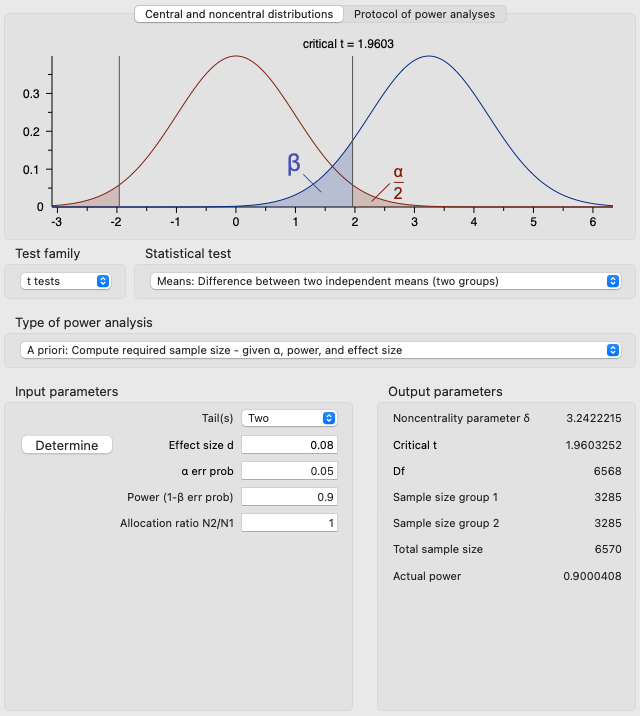
\includegraphics[width=0.9\linewidth]{0_TwoSamplePowerAnalysis.png}
    \caption{Power analysis with G*Power}
    \label{fig:gpower-power-analysis}
\end{figure}



\end{appendix}

\end{document}